% Template from latex.tugraz.at

\documentclass[%
%handout, % prints handouts (=no animations, for printed version)
%mathserif
%xcolor=pst,
14pt
% fleqn
]{beamer}

\usepackage{beamerthemedefault}

\useoutertheme[subsection=false]{smoothbars}
\useinnertheme[shadow=true]{rounded}

\setbeamercolor{block title}{fg=black,bg=gray}
\setbeamercolor{block title alerted}{use=alerted text,fg=black,bg=alerted text.fg!75!bg}
\setbeamercolor{block title example}{use=example text,fg=black,bg=example text.fg!75!bg}
\setbeamercolor{block body}{parent=normal text,use=block title,bg=block title.bg!25!bg}
\setbeamercolor{block body alerted}{parent=normal text,use=block title alerted,bg=block title alerted.bg!25!bg}
\setbeamercolor{block body example}{parent=normal text,use=block title example,bg=block title example.bg!25!bg}

\setbeamertemplate{itemize item}{\textbullet}
\setbeamertemplate{itemize subitem}{\textbullet}

%% for including video/audio
%\usepackage{multimedia} %needs hyperref-package

%% aktive Referenzen
\usepackage{hyperref}

%\usepackage{ngerman}			% language set to new-german
\usepackage[english]{babel}
\usepackage[utf8]{inputenc} 	% coding of german special characters
% \usepackage{ae,aecompl}
% \usepackage{amsmath,amssymb,amstext} 	% support for mathematics

% \usepackage{listings}		% include programming code
%\usepackage{amsfonts}		% blackboard fonts: $\mathbb{N,Z,R,C,...}$
%\usepackage{latexsym}
%\usepackage{textcomp}
%\usepackage{mathptmx,courier}
			% \textdegree \textcelsius \textperthousand
			% \copyright \texttrademark \textregistered
			% \textmu (non-italic mu)
%\usepackage{geometry}	% change paper dimension an margins
%    \geometry{verbose,paperwidth=128mm,paperheight=90mm}
%    \geometry{tmargin=0mm,bmargin=0mm,lmargin=10mm,rmargin=10mm}
%\usepackage{graphicx}  % \includegraphics[options]{file.eps}
			% options = scale, width, totalheight, height, depth,
			% angle = deg, origin = {l c r}{top, Baseline, bottom}
			% \scalebox{h-scale}[v-scale]{object}
			% \rotatebox[x=xdim,y=ydim]{angleCCW}[object}
%\usepackage{tabularx}	% \begin{tabular}{...X...} stretches column
%\usepackage{multirow}
%\usepackage{floatflt}
%\usepackage{hhline}
%\usepackage{colortbl}
\usepackage{array}
\usepackage{setspace}
\usepackage{textcomp}
\usepackage{subfigure}

%\usepackage[thinspace,thinqspace,squaren,textstyle]{SIunits}

\definecolor{tug}{rgb}{0.96862,0.14509,0.27450}

\setbeamertemplate{headline}[text line]{
	\begin{beamercolorbox}[wd=\paperwidth,ht=8ex,dp=4ex]{}
		\insertnavigation{0.85\paperwidth} 
		\raisebox{-10pt}{
\includegraphics[width=15mm]{tuglogo}}\vskip2pt
		\hskip-1pt\rule{\paperwidth}{0.3pt}
	\end{beamercolorbox}
}

\setbeamertemplate{navigation symbols}{}

\definecolor{gray}{rgb}{0.8,0.8,0.8}
\setbeamercolor{footline}{fg=black,bg=gray}

% Fußzeile mit Autor, Titel und Foliennummer / Gesamtfolienzahl
\setbeamertemplate{footline}[text line]{
	\hskip-1pt
	\begin{beamercolorbox}[wd=\paperwidth]{footline}
			\rule{\paperwidth}{0.3pt}
			\colorbox{tug}{\rule{3pt}{0pt}\rule{0pt}{3pt}}
			\textbf{\rule{0pt}{5pt}\insertshortauthor\hfill\insertshortinstitute\hfill%
					\insertshorttitle\rule{1em}{0pt}}
			\rule{\paperwidth}{0.3pt}
	\end{beamercolorbox}
	\begin{beamercolorbox}[wd=\paperwidth,ht=2ex,dp=2ex]{white}
	\end{beamercolorbox}
}%

\newtheorem{idea}{Idea}


%% Titelblatt-Einstellungen
\title{Implementation of an Evolutionary Optimization Framework \\%}
%\subtitle{
and Application to the Open Job Shop Problem}
\author{Joris Bayer, Stefan Kroboth}
% \date{}		% wenn ein anderes als das heutige Datum eingesetzt werden soll

% Subject und Keywords für PDF-Datei
\subject{Implementation of an Evolutionary Optimization Framework and Application to the Open Job Shop Problem}
\keywords{Numerical Optimization, Evolutionary Algorithms, Open Job Shop Problem}

\titlegraphic{
\includegraphics[width=20mm]{tuglogo}}

%%%%%%%%%%%%%%%%%%%%%%%%%%%%%%%%%%%%%%%%%%%%%%%%%%%%%%%%%%%%%%%%%%%%%%%%%%%%
\begin{document}
%%%%%%%%%%%%%%%%%%%%%%%%%%%%%%%%%%%%%%%%%%%%%%%%%%%%%%%%%%%%%%%%%%%%%%%%%%%%

\begin{frame}[plain]
  \frametitle{}
  \titlepage % erzeugt Titelseite
\end{frame}



% \begin{frame}
%   \frametitle{Content}
%         %\tableofcontents[hideallsubsections %
%                         % ,pausesections
%         %                ] % erzeugt Inhaltsverzeichnis
% \end{frame}

\section{Introduction}
\subsection{nix}
\begin{frame}
  \frametitle{Motivation}
  \begin{itemize}
    \item Implementation of an evolutionary optimization framework in Julia
    \item Generalized design to solve a wide range of problems
    \item Make it easy to build algorithms on top of the framework
    \item Evaluation of the framework with an interesting problem (Open Job Shop)
  \end{itemize}
\end{frame}


\begin{frame}
	
	\frametitle{Evolutionary Basics}
%	\vspace{-1cm}
	\begin{figure}[htbp]
		\centering
			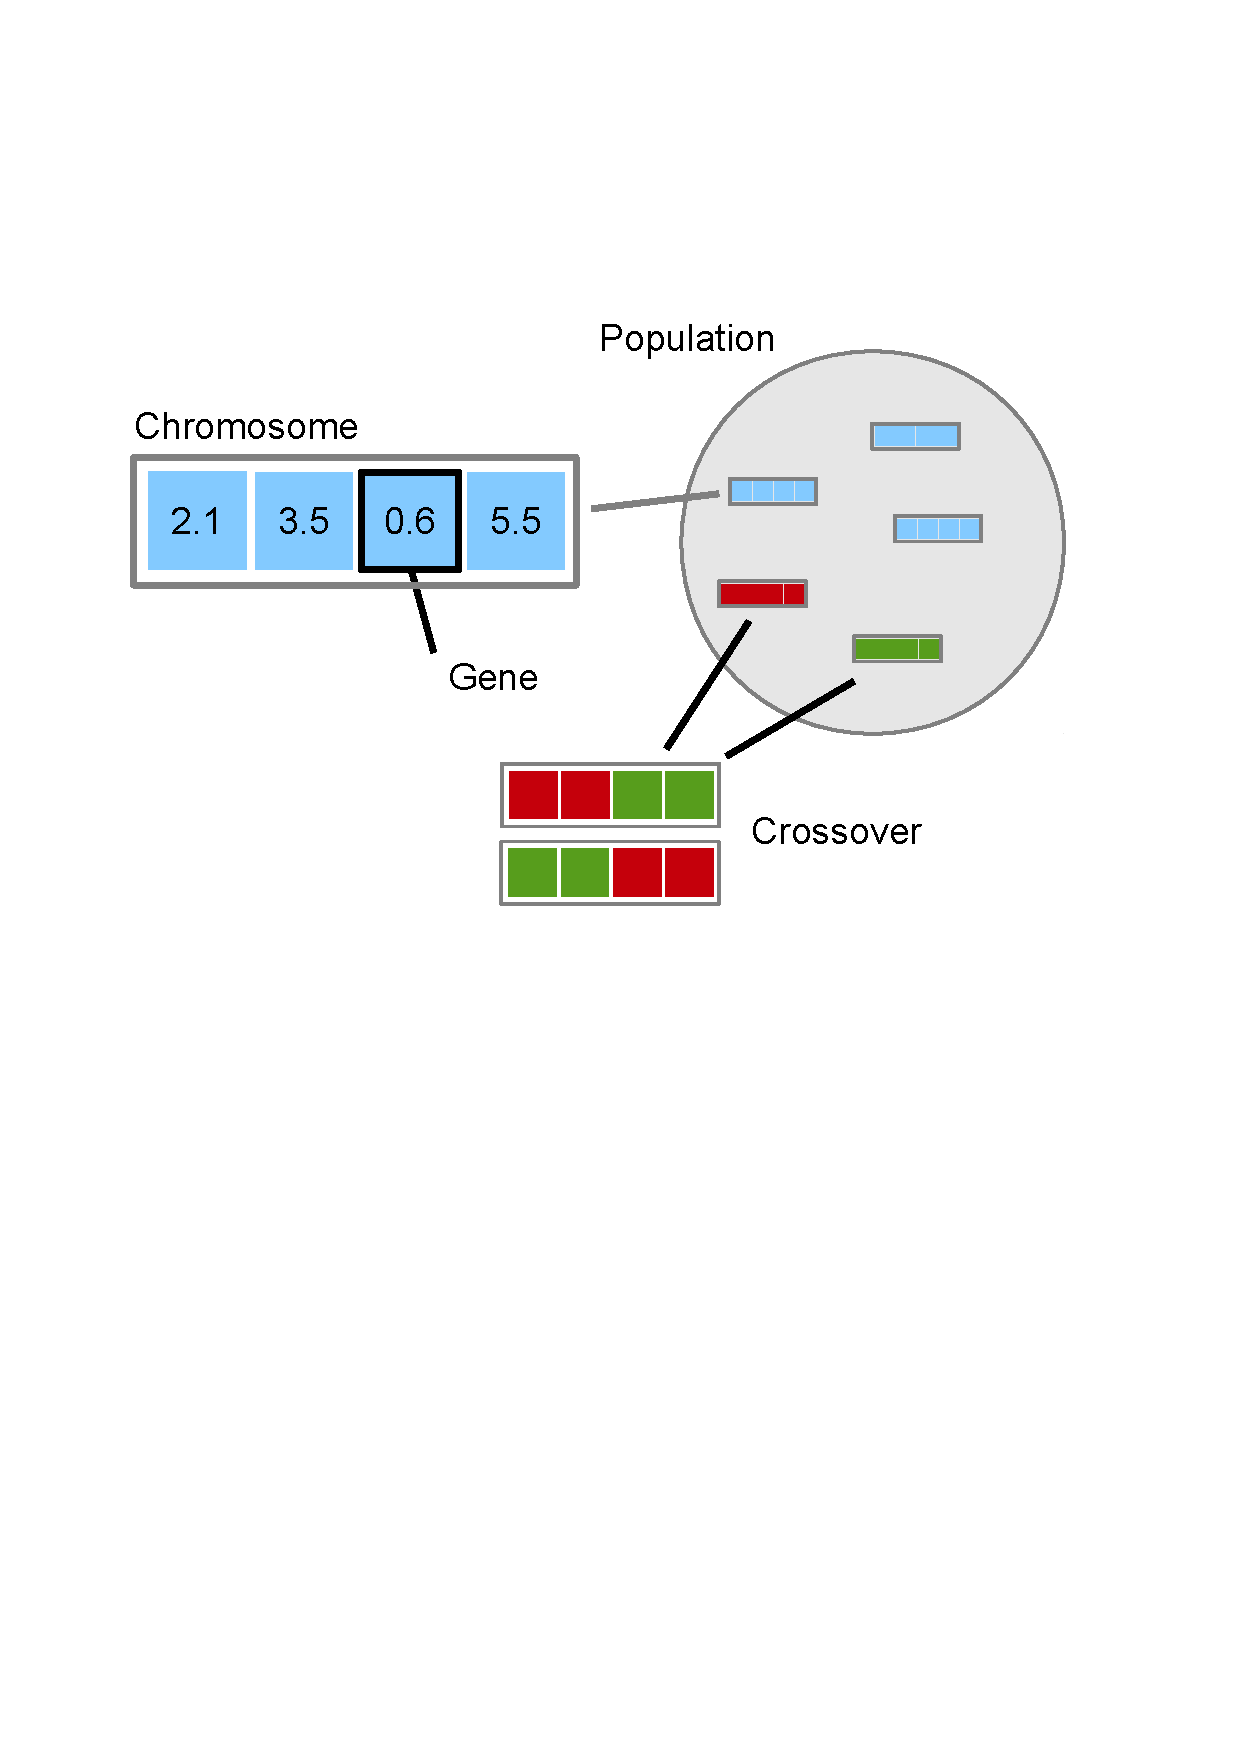
\includegraphics[scale=.6]{images/evo-basics.pdf}
%		\caption{caption}
		\label{fig:label}
	\end{figure}
\end{frame}


\begin{frame}
  \frametitle{The Julia Language}
  \begin{itemize}
    \item high-level, high-performance dynamic programming language for technical computing
    %\item Syntax similar to \textsc{Matlab} and Python
    \item just in time (JIT) compilation (using LLVM)
    %\item aggressive optimization
    \item optional typing
    \item multiple dispatch
    %\item Lisp-like macro system
    \item often C-like performance
    \item easy distributed and parallel computing
  \end{itemize}
\end{frame}

\section{evolib}
\subsection{nix}
\begin{frame}
  \frametitle{evolib - A Julia Library}
  \begin{itemize}
    \item Makes heavy use of multiple dispatch
    \item Defines types \texttt{Gene}, \texttt{Chromosome}, \texttt{Population} and \texttt{Generation}
    %\item Types are exchangeable due to Type hierarchy
    \item Lots of convenience functions
      %\begin{itemize}
        %\item Constructors for each type
        %\item Generate random instances of types
        %\item Indexing and modifiers
        %\item Roulette Wheel Selection
        %\item Mutation, Crossover
      %\end{itemize}
    \item Basic genetic and evolutionary algorithms based on these types
  \end{itemize}
\end{frame}

\subsection{Algorithms}
\begin{frame}
  \frametitle{Algorithms}
  \begin{spacing}{1.5}
    \begin{itemize}
      \item Implemented as displayed in the lecture notes:
        \begin{itemize}
          \item Genetic Algorithm
          \item (1+1) Evolutionary Strategy
          \item $(\mu/\rho, \lambda)$ Evolutionary Strategy
        \end{itemize}
    \end{itemize}
  \end{spacing}
\end{frame}

\begin{frame}[fragile]
  \frametitle{Example}
  \vspace{-0.5cm}
{\scriptsize
\begin{verbatim}
load("evolib.jl")

function rosenbrock(chr::Chromosome)
    x1 = chr[1].gene
    x2 = chr[2].gene
    chr.fitness = 100*(x2-x1^2)^2+(1-x1)^2-50*((x1+1)^2+(x2-1)^2)
                 -10*((x1-1.5)^2+(x2-2.5)^2)+exp(2*x2-5)
end

function rosenbrock(pop::Population)
    for i=1:length(pop)
        rosenbrock(pop[i])
    end
end

popul = rand(Population, 100, 2, rosenbrock, 1.0, 6.0, -6.0 )

@time best = evo_slash(popul, 2, 150, 1000, 0.85, 0.0000001, rosenbrock)
print(best)

\end{verbatim}}
\end{frame}

\section{Open Job Shop Problem}

%%%%%%%%%%%%%%%%%%%%%%%%%%%%%%%%%%%%%%%%%%%%%%%%%%%%%%%%%%%%%%%%%%%%%%%%%%%%%%%%
\subsection{Introduction}

%%%%%%%%%%%%%%%%%%%%%%%%%%%%%%%%%%%%%%%%%%%%%%%%%%%%%%%%%%%%%%%%%%%%%%%%%%%%%%%%


\begin{frame}
  \frametitle{Open Job Shop Scheduling Problem}

  \begin{itemize}
    \item $m$ \textbf{jobs} have to processed by $n$ \textbf{machines}
    \item A job $i$ stays on a machine $j$ for an \textbf{operation} with start time $t_{ij}$ and duration $d_{ij}$
    \item The order in which a job is passed from machine to machine can be chosen arbitrarily.
  \end{itemize}

  Goal: \textbf{minimize} the total \textbf{makespan}, i.e. the time at which the last machine finishes its last operation.

 	

\end{frame}

%%%%%%%%%%%%%%%%%%%%%%%%%%%%%%%%%%%%%%%%%%%%%%%%%%%%%%%%%%%%%%%%%%%%%%%%%%%%%%%%

\begin{frame}
	\frametitle{Example}
	
	\begin{columns}[c]
		\column{.4\linewidth}

Valid schedule for a 3x3-problem (3 jobs, 3 machines)

\textbf{makespan:} 23, matches lower bound

		\column{.6\linewidth}
		\vspace{-1cm}
\begin{figure}
	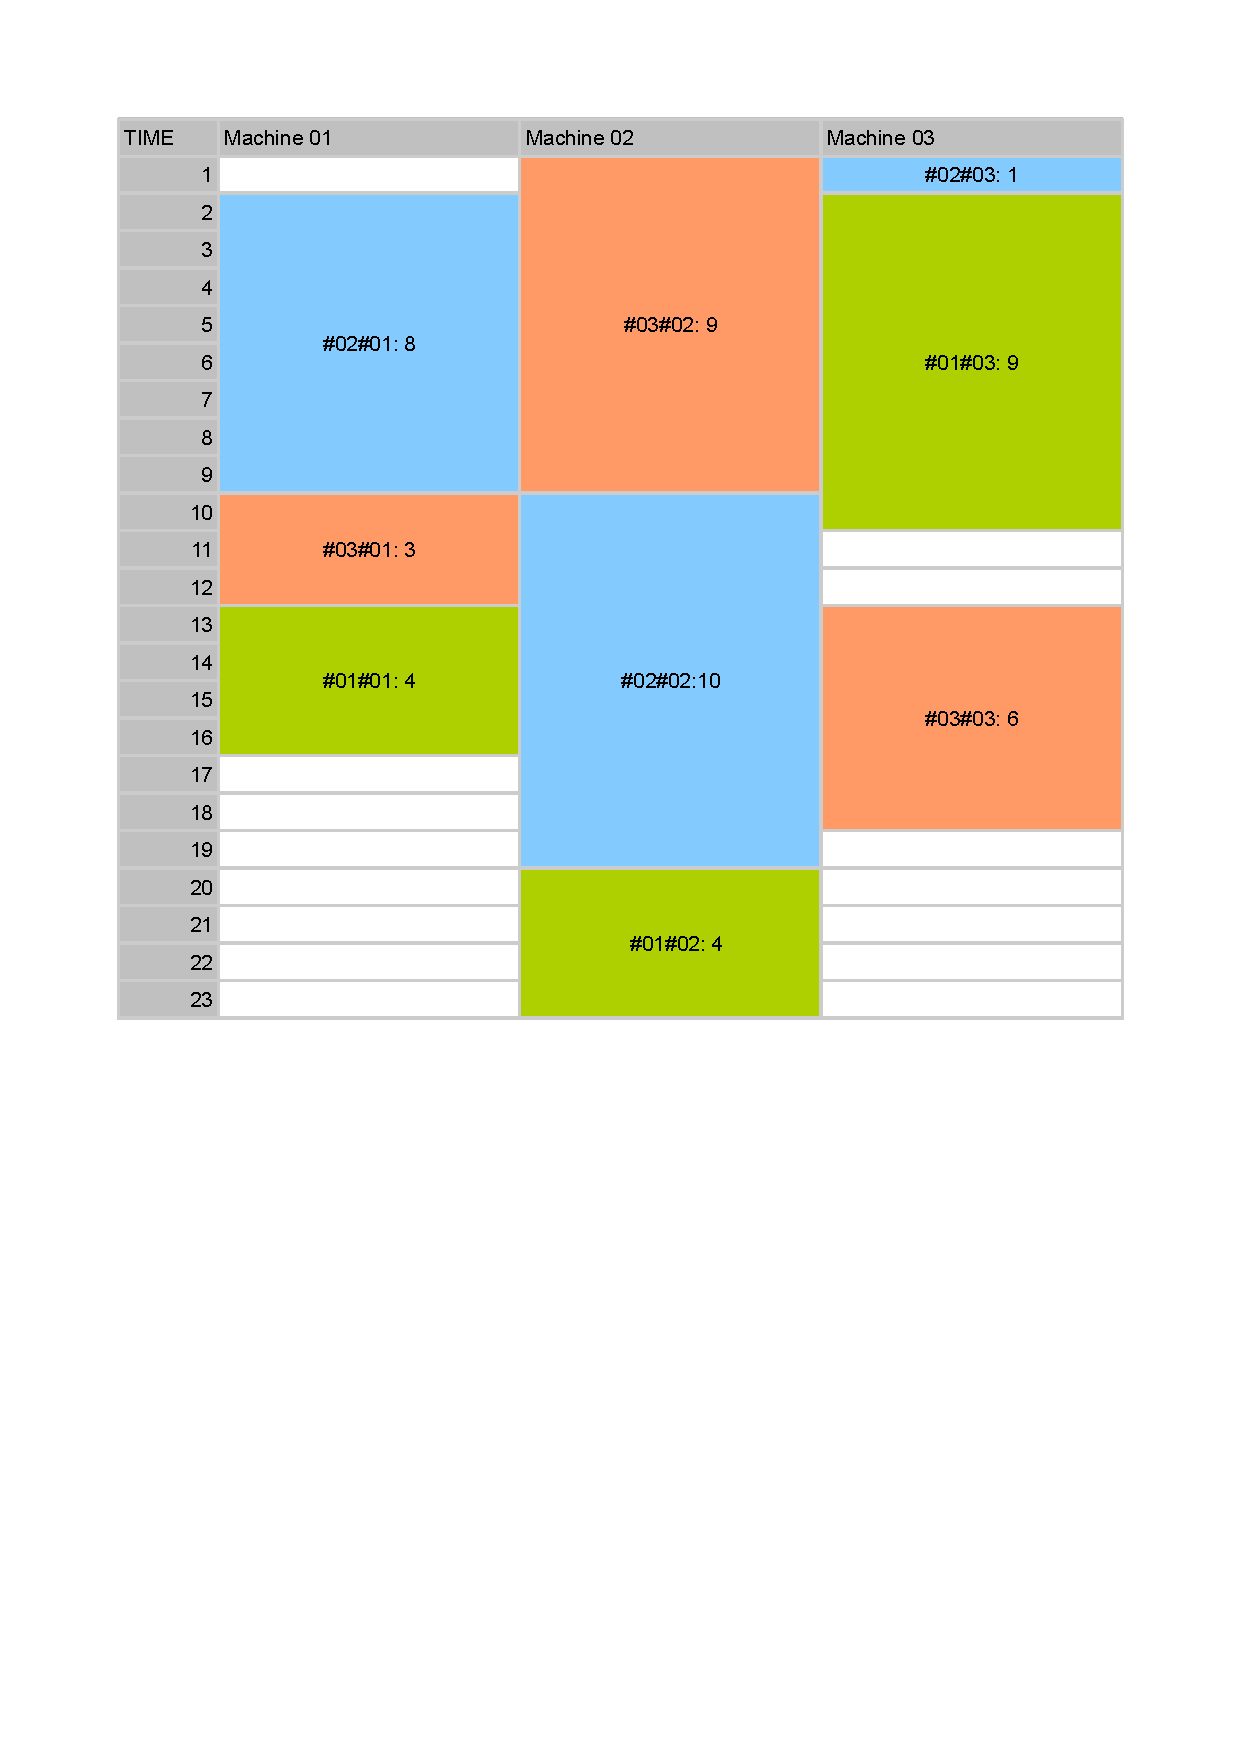
\includegraphics[width=\linewidth]{images/example-schedule.pdf}
	
\end{figure}
\end{columns}
	
\end{frame}

%%%%%%%%%%%%%%%%%%%%%%%%%%%%%%%%%%%%%%%%%%%%%%%%%%%%%%%%%%%%%%%%%%%%%%%%%%%%%%%%

\begin{frame}
	\frametitle{$NP$-hardness}
	
	\begin{itemize}
	
		\item Similar to normal Job Shop and Flow Shop problems, but with a larger solution space \textrightarrow \hspace{.5em} harder to find optimal solution.

		\item 	The Open Job Shop Scheduling Problem is known to be $NP$-hard for $n \geq 3$ (the Partitioning Problem can be reduced to it).

		\item 	\textrightarrow \hspace{.5em} Research focuses on \textbf{heuristics} since exact approaches are not feasible.
	\end{itemize}
	
	
\end{frame}

%%%%%%%%%%%%%%%%%%%%%%%%%%%%%%%%%%%%%%%%%%%%%%%%%%%%%%%%%%%%%%%%%%%%%%%%%%%%%%%%

\begin{frame}
	\frametitle{Known Approaches}
	\begin{itemize}
	
		\item Branch and Bound (1997)

		\item 	Tabu Search (1999)

		\item 	\textbf{Evolutionary based heuristics} (1999)

		\item 	Particle Swarm Optimization (2008)
	\end{itemize}
	
	
\end{frame}

%%%%%%%%%%%%%%%%%%%%%%%%%%%%%%%%%%%%%%%%%%%%%%%%%%%%%%%%%%%%%%%%%%%%%%%%%%%%%%%%

\subsection{Algorithms}

%%%%%%%%%%%%%%%%%%%%%%%%%%%%%%%%%%%%%%%%%%%%%%%%%%%%%%%%%%%%%%%%%%%%%%%%%%%%%%%%

\begin{frame}
  \frametitle{Permutation Genetic Algorithm}
	
	\begin{idea}
	
	
	\begin{itemize}
	
		\item Give each operation a unique $ID = 1,2,\dots, m \cdot n$

		\item 	Let the order of the IDs decide which operation is \textbf{scheduled} first.

		\item 	Use the \emph{genetic algorithm} to find the best \emph{permutation}.
	\end{itemize}
	
	\end{idea}
	
	\pause
	
	What does it mean to \emph{schedule} an operation?  

\end{frame}

%%%%%%%%%%%%%%%%%%%%%%%%%%%%%%%%%%%%%%%%%%%%%%%%%%%%%%%%%%%%%%%%%%%%%%%%%%%%%%%%

\begin{frame}
  \frametitle{Scheduling step}
	
	
	\small
	\begin{columns}	
	\column{.5\textwidth}
Simple scheduling: Append operation to machine, after previous operations of the same job have finished.



\column{.5\linewidth}
	\begin{figure}
		\centering
		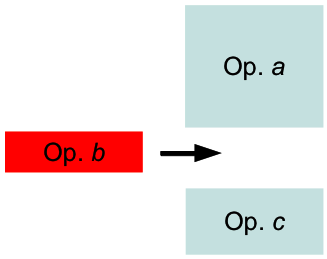
\includegraphics[width=.8\linewidth]{images/scheduling.png}

	\end{figure}
	
\end{columns}

\textbf{Better:} Use \textbf{gaps} (no other operation of the same job should be active)!

	A significant part of the optimization is ``hidden'' in this scheduling step!

\end{frame}

%%%%%%%%%%%%%%%%%%%%%%%%%%%%%%%%%%%%%%%%%%%%%%%%%%%%%%%%%%%%%%%%%%%%%%%%%%%%%%%%

\begin{frame}
    \frametitle{Implementation details}
    \begin{itemize}

    	\item A chromosome consists of $m\cdot~n$ genes, each gene representing an operation.

    	\item Start with random genes

    	\item Genetic algorithm adapts genes freely as floats \textrightarrow \hspace{.5em} the order of the genes decides the permutation, e.g.

    	\item a chromosome $(64.4, 33.5, 64.5)$ represents the permutation $(2,1,3)$
    \end{itemize}
\end{frame}

%%%%%%%%%%%%%%%%%%%%%%%%%%%%%%%%%%%%%%%%%%%%%%%%%%%%%%%%%%%%%%%%%%%%%%%%%%%%%%%%

\begin{frame}
  \frametitle{Hybrid Genetic Algorithm}
\begin{itemize}

	\item 	Uses the same genetic algorithm with the same parameters, but

	\item  	permutes jobs instead of operations

	\item 	Called \textbf{hybrid}, because it keeps a sorted list of unfinished operations for each job \textrightarrow \hspace{.5em} schedules long operations first
	
\end{itemize}


 
\end{frame}


%%%%%%%%%%%%%%%%%%%%%%%%%%%%%%%%%%%%%%%%%%%%%%%%%%%%%%%%%%%%%%%%%%%%%%%%%%%%%%%%

\begin{frame}
  \frametitle{Hybrid Genetic - Example}

\begin{figure}[htbp]
	\centering
		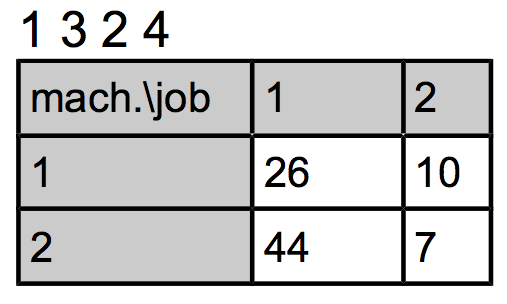
\includegraphics[scale=1]{images/hyb0.png}
	\caption{The table represents the problem definition, the sequence ``1 3 2 4'' directs the scheduling order.}
	\label{fig:label}
\end{figure}
	
 
\end{frame}
\begin{frame}
  \frametitle{Hybrid Genetic - Example (1)}

\begin{figure}[htbp]
	\centering
		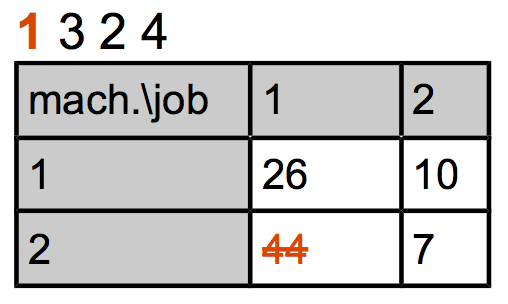
\includegraphics[scale=1]{images/hyb1.png}
	\caption{First, schedule the longest operation of job 1 (left column).}
	\label{fig:label}
\end{figure}
	
 
\end{frame}
\begin{frame}
  \frametitle{Hybrid Genetic - Example (2)}

\begin{figure}[htbp]
	\centering
		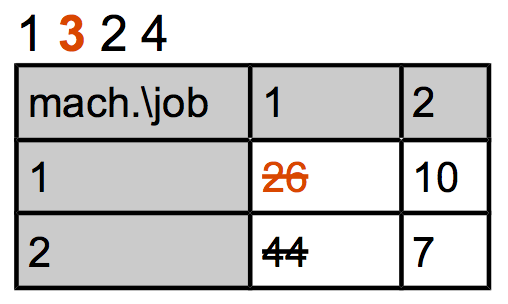
\includegraphics[scale=1]{images/hyb2.png}
	\caption{The index 3 also points to job 1 (modulo). Schedule the second longest operation.}
	\label{fig:label}
\end{figure}
	
 
\end{frame}
\begin{frame}
  \frametitle{Hybrid Genetic - Example (3)}

\begin{figure}[htbp]
	\centering
		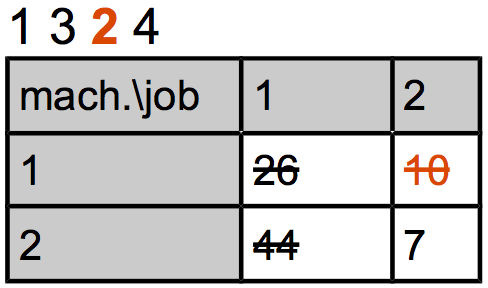
\includegraphics[scale=1]{images/hyb3.png}
	\caption{Now, any index would refer to job 2, because it's the only unfinished job. Schedule the longest operation.}
	\label{fig:label}
\end{figure}
	
 
\end{frame}
\begin{frame}
  \frametitle{Hybrid Genetic - Example (4)}

\begin{figure}[htbp]
	\centering
		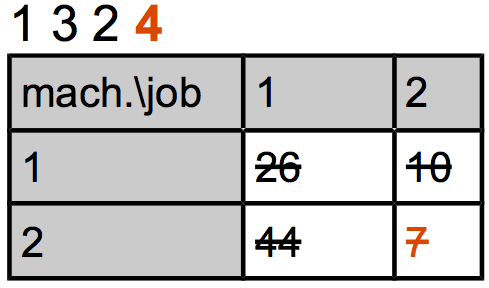
\includegraphics[scale=1]{images/hyb4.png}
	\caption{Finish scheduling.}
	\label{fig:label}
\end{figure}
	
 
\end{frame}

%%%%%%%%%%%%%%%%%%%%%%%%%%%%%%%%%%%%%%%%%%%%%%%%%%%%%%%%%%%%%%%%%%%%%%%%%%%%%%%%

\begin{frame}
  \frametitle{Selfish Gene Algorithm}

\begin{itemize}

	\item Uses a \textbf{virtual population} (VP)%, does \textbf{not} use the evolib!

	\begin{itemize}
		\item instead of storing chromosomes, store probabilities of gene values.

		\item Indivuals are drawn from the VP according to these probabilities.

		\item Better fitness means higher probability for genes (a competition is held).
	
		\item \textbf{steady state}: Every gene acquires a certain value with  $P \geq 95\%$.
	\end{itemize}
	\item In our case: genes represent job/machine indices.
\end{itemize}

\end{frame}

%%%%%%%%%%%%%%%%%%%%%%%%%%%%%%%%%%%%%%%%%%%%%%%%%%%%%%%%%%%%%%%%%%%%%%%%%%%%%%%%

\begin{frame}[fragile]
	\frametitle{Selfish Gene Algorithm - Pseudocode}
	
\vspace{-0.8cm}
{\scriptsize
\begin{verbatim}
SELFISH_GENE():
    
    population = [[1/m,1/n,...],[1/m,1/n,...], ...]
    best = choose individual from population
    
    FOR i = 1:max_iterations
        choose individual1, individual2 from population
        (winner, loser) = compare(individual1, individual2)
        reward(winner)
        punish(loser)
        IF fitness(winner) > fitness(best)
            best = winner
        END
        BREAK if steady_state(population)
    END
    
    RETURN best
\end{verbatim}}

\end{frame}

%%%%%%%%%%%%%%%%%%%%%%%%%%%%%%%%%%%%%%%%%%%%%%%%%%%%%%%%%%%%%%%%%%%%%%%%%%%%%%%%


\section{Evaluation}

%%%%%%%%%%%%%%%%%%%%%%%%%%%%%%%%%%%%%%%%%%%%%%%%%%%%%%%%%%%%%%%%%%%%%%%%%%%%%%%%
\subsection{nix}
%%%%%%%%%%%%%%%%%%%%%%%%%%%%%%%%%%%%%%%%%%%%%%%%%%%%%%%%%%%%%%%%%%%%%%%%%%%%%%%%
\begin{frame}
  \frametitle{Evaluation}
\begin{itemize}

	\item We wanted to rigorously compare our results with the results from the original paper.
	\item But: no implicit datasets available!

	\item We had to implement a special random number generator (RNG) and a benchmark generator from pseudocode delivered by \cite[Taillard'03]{Benchmarks}.

	\item The benchmarks were reproduced based on given seeds for the RNG.
\end{itemize}

\end{frame}

%%%%%%%%%%%%%%%%%%%%%%%%%%%%%%%%%%%%%%%%%%%%%%%%%%%%%%%%%%%%%%%%%%%%%%%%%%%%%%%%

\begin{frame}
	\frametitle{Evaluation method}
\begin{itemize}

	\item We considered benchmark problems of sizes
		\begin{itemize}
		
			\item 4x4 (4 jobs, 4 machines), 5x5, 7x7, 10x10, 15x15, 20x20. 
		\end{itemize}
		
	For each problem, we  ran all 3 algorithms for \textbf{200} generations with a population size of \textbf{200}.

	\item 	Since different runs produce different results, we repeated each run \textbf{100} times. 
	\\ 		\textcolor{red}{\textrightarrow		High computational cost!}

	\item 	Complexity increases with rising problem size \textrightarrow	only a few large problems evaluated 
\end{itemize}

	
\end{frame}

%%%%%%%%%%%%%%%%%%%%%%%%%%%%%%%%%%%%%%%%%%%%%%%%%%%%%%%%%%%%%%%%%%%%%%%%%%%%%%%%
%\subsection{Results}
%%%%%%%%%%%%%%%%%%%%%%%%%%%%%%%%%%%%%%%%%%%%%%%%%%%%%%%%%%%%%%%%%%%%%%%%%%%%%%%%

\begin{frame}
  \frametitle{Results}
	\vspace{-1.8cm}
\begin{figure}[htbp]
	\centering
	\hspace{1cm}
		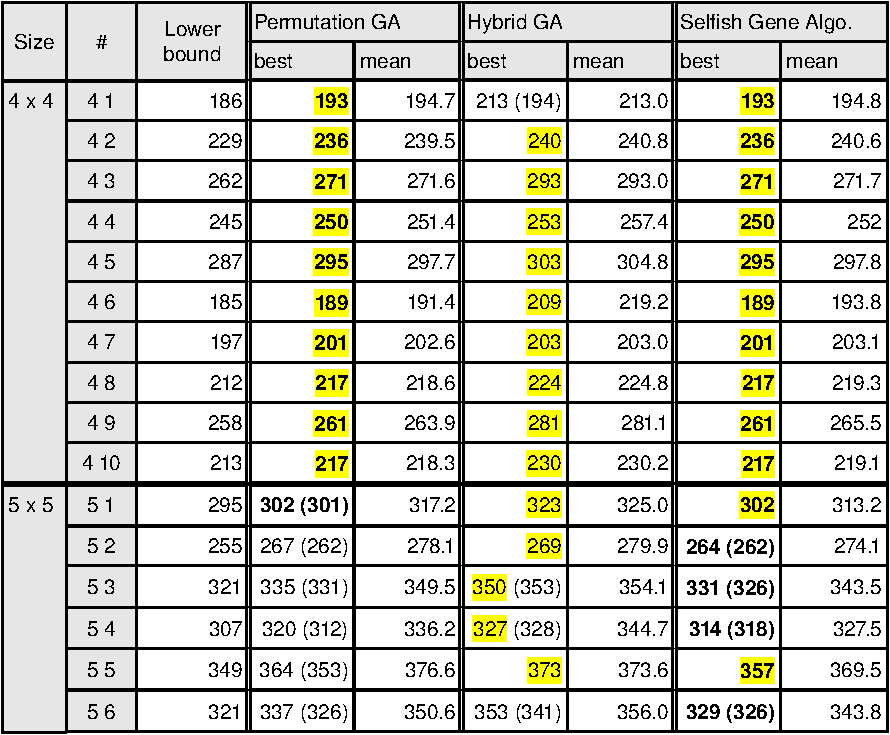
\includegraphics[scale=.5]{images/results1.pdf}
	\caption{We reached the best known solution for all 4x4 problems. For medium problems (5x5, 7x7), the Selfish Gene Algorithm performs best.}
	\label{fig:label}
\end{figure}
\end{frame}

%%%%%%%%%%%%%%%%%%%%%%%%%%%%%%%%%%%%%%%%%%%%%%%%%%%%%%%%%%%%%%%%%%%%%%%%%%%%%%%%

\begin{frame}
  \frametitle{Results (2)}

\begin{figure}[htbp]
	\centering
		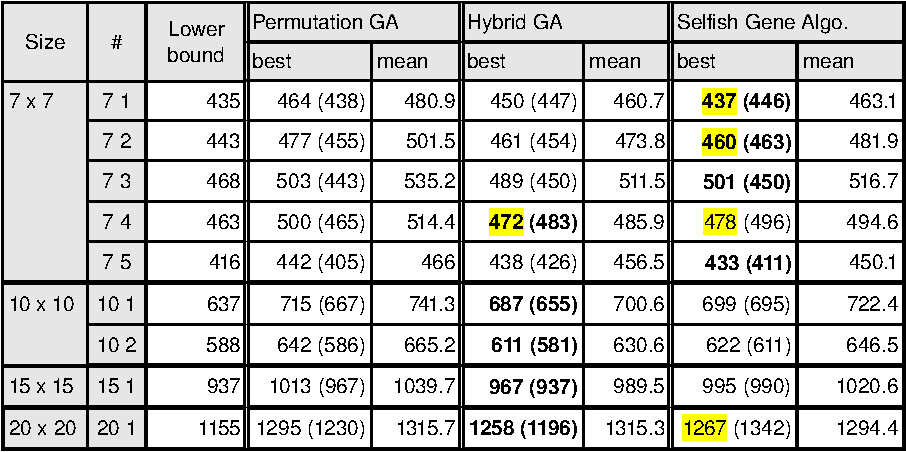
\includegraphics[scale=.5]{images/results2.pdf}
	\caption{The gap between lower bounds and found solutions increases with the problem size. For large problems, the hybrid GA performs best.}
	\label{fig:label}
\end{figure}
\end{frame}

%%%%%%%%%%%%%%%%%%%%%%%%%%%%%%%%%%%%%%%%%%%%%%%%%%%%%%%%%%%%%%%%%%%%%%%%%%%%%%%%

\begin{frame}
	\frametitle{Results (3)}
\begin{itemize}

	\item 	We matched the best known results for small problems.

	\item 	We found acceptable solutions for larger problems, but
		\begin{itemize}
			\item 		we implemented our own library instead of using a well known optimization library
			\item 		therefore implementations of functions like \emph{crossover} may differ
		\end{itemize}
		

	\item 	Neither our nor the original implementation matched the results of \cite[PSO'08]{PSO}.
\end{itemize}

	
\end{frame}

%%%%%%%%%%%%%%%%%%%%%%%%%%%%%%%%%%%%%%%%%%%%%%%%%%%%%%%%%%%%%%%%%%%%%%%%%%%%%%%%

\begin{frame}
  \frametitle{Convergence: 4x4 Problem}
  \begin{figure}[htbp]
    \centering
    \subfigure[Permutation GA]{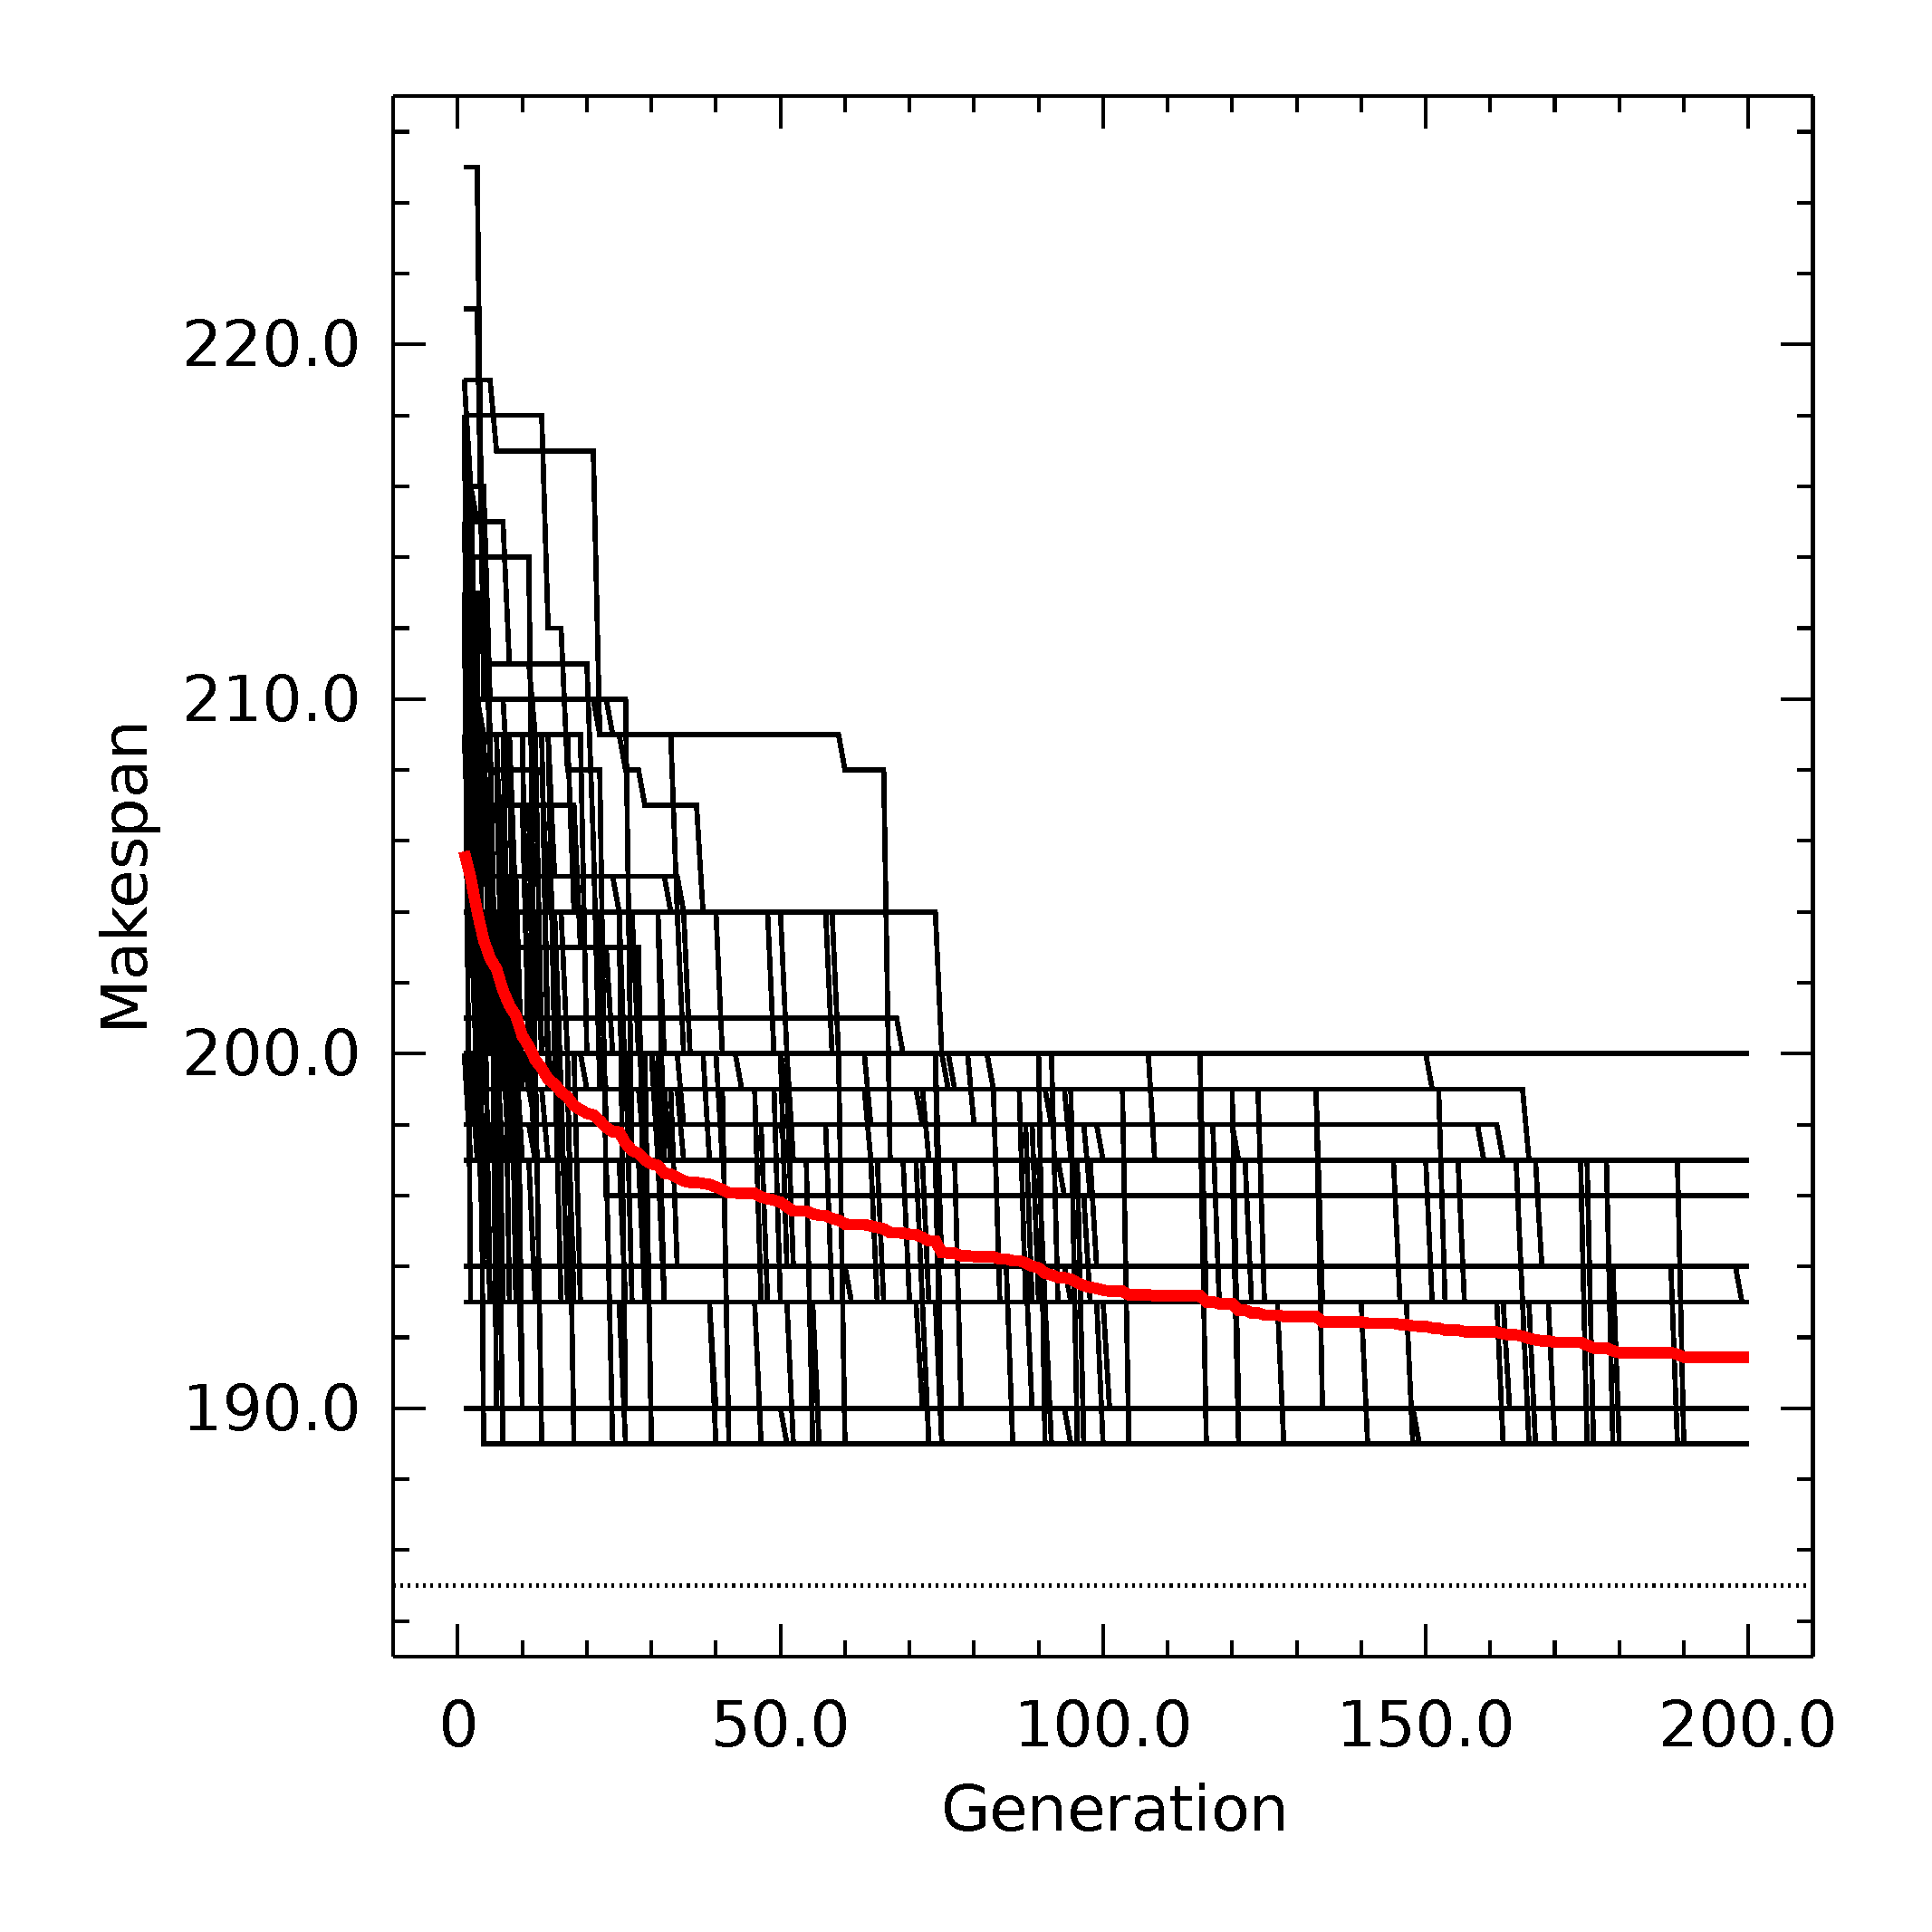
\includegraphics[scale=.095]{../open_jobshop/output/perm_4_6_200.pdf}}
    \subfigure[Hybrid GA]{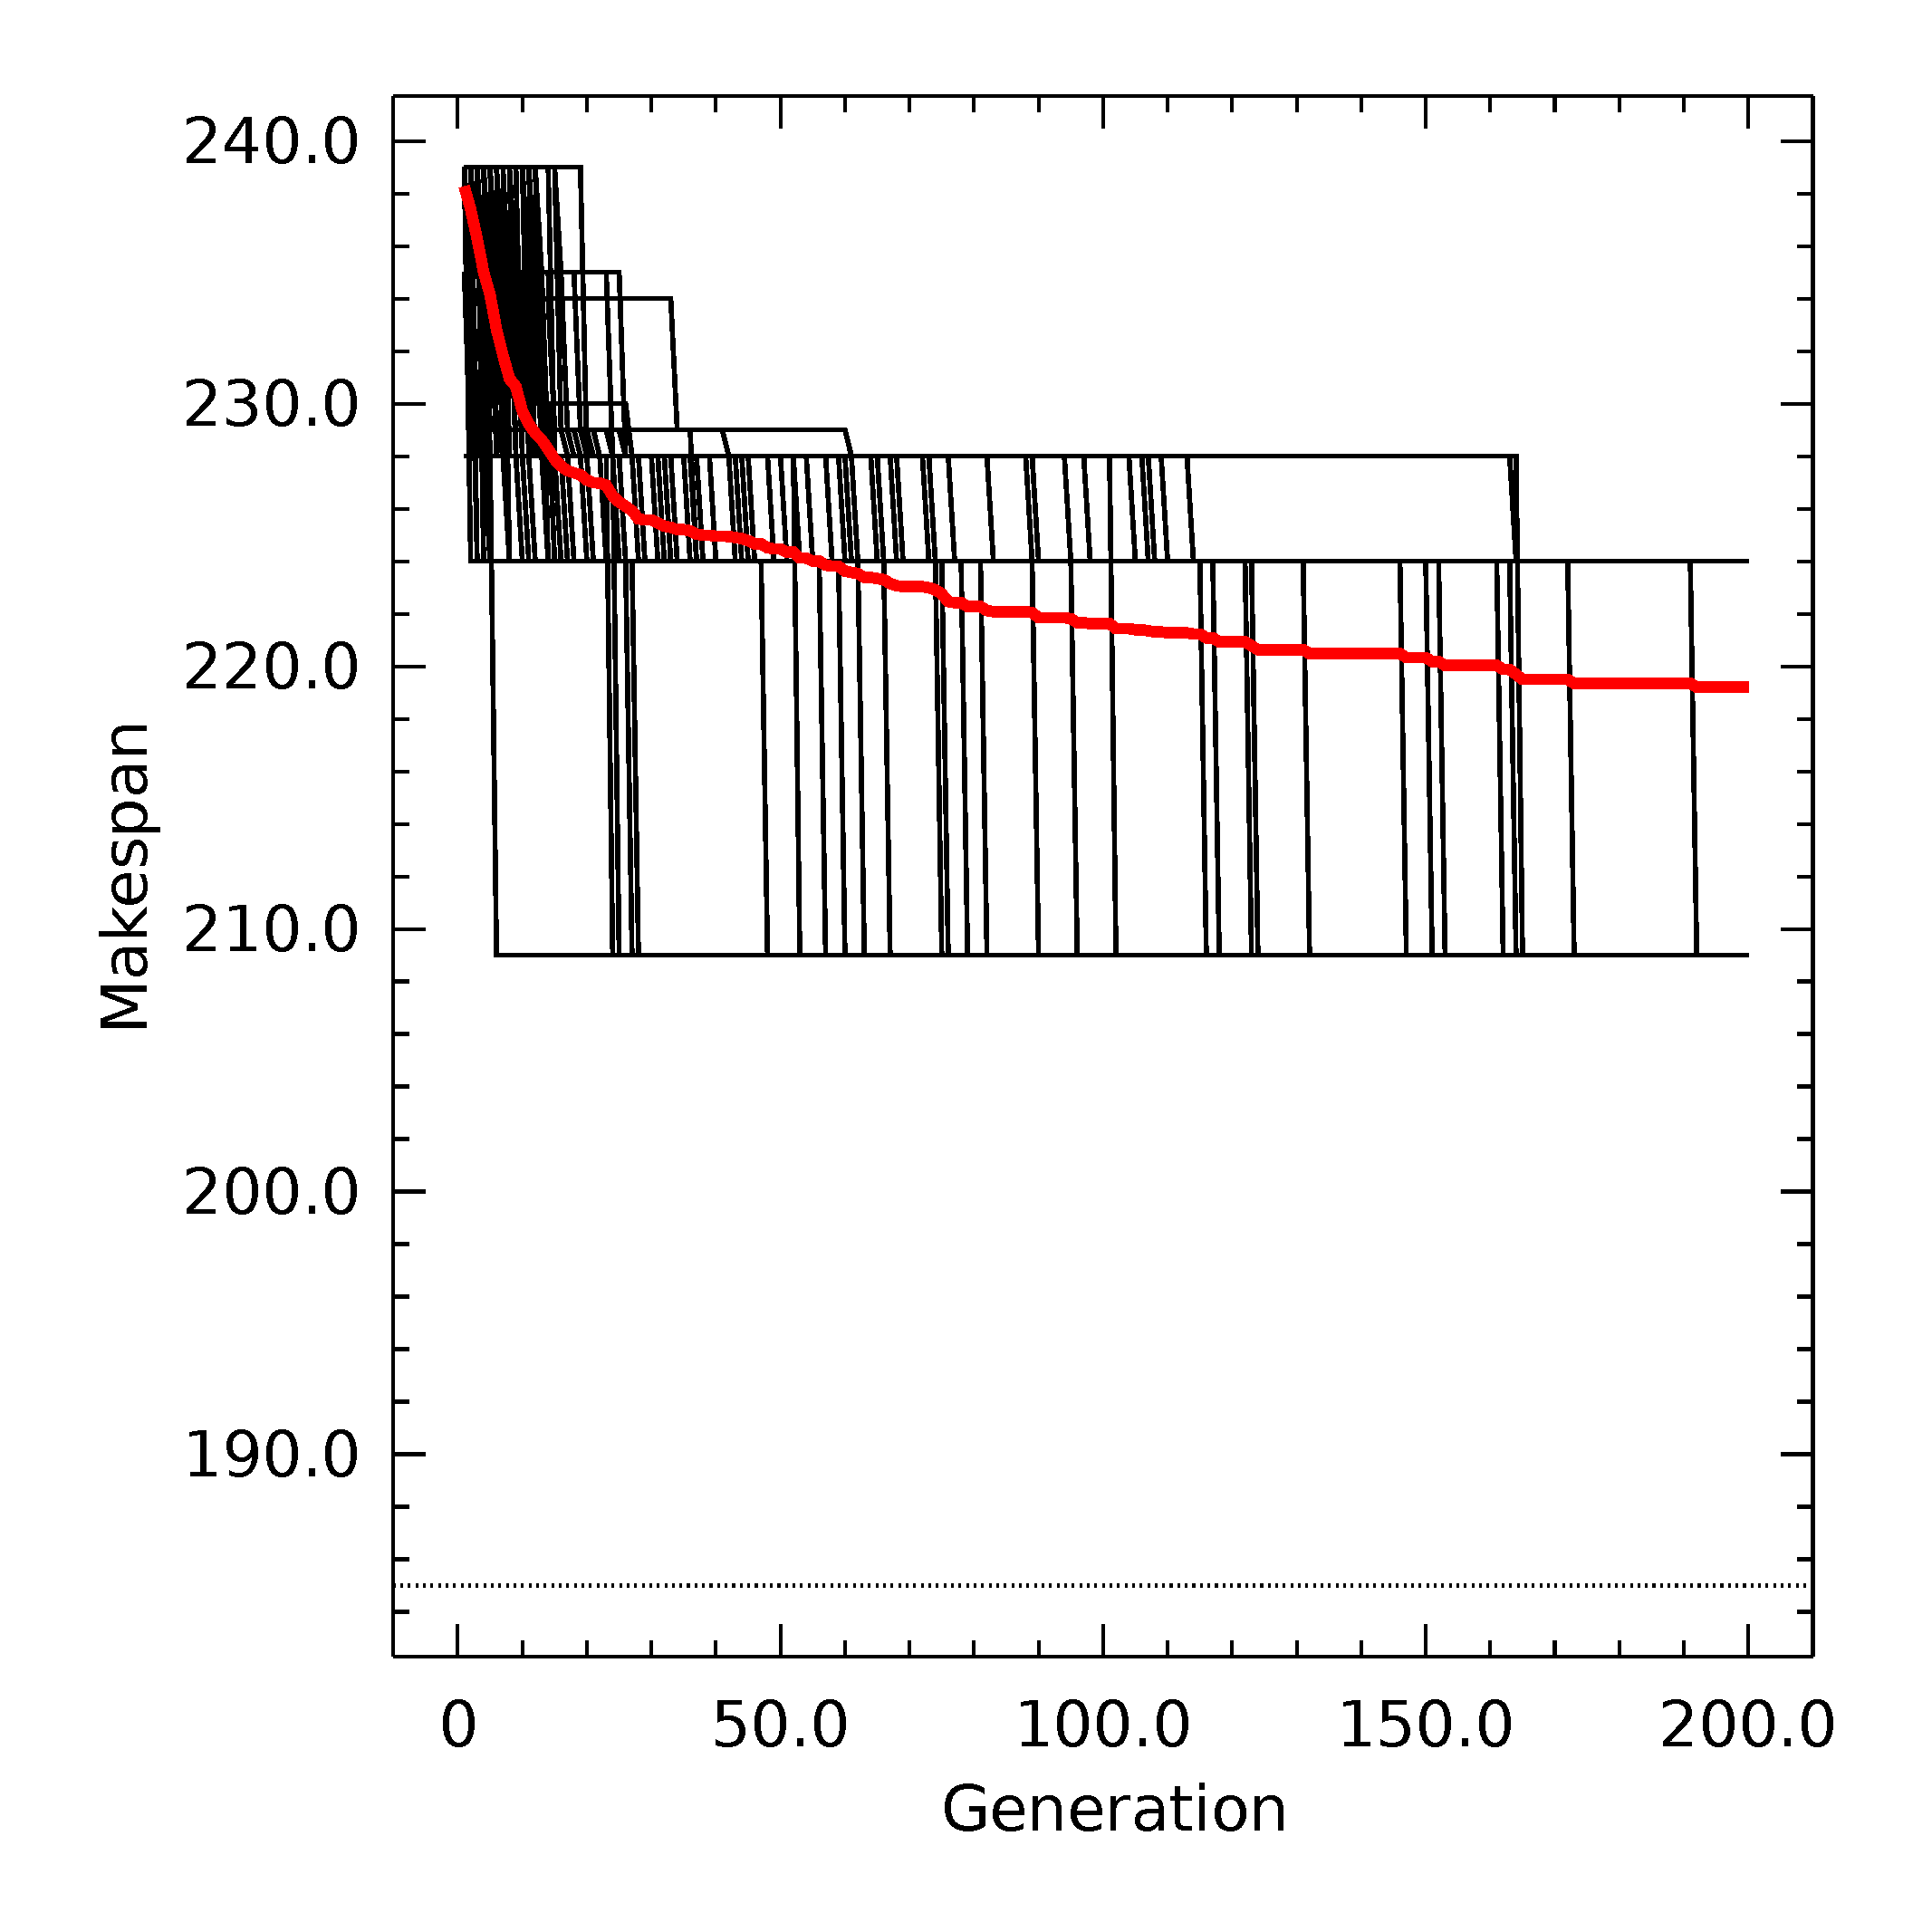
\includegraphics[scale=.095]{../open_jobshop/output/hyb_4_6_200.pdf}}
    \subfigure[Selfish Gene]{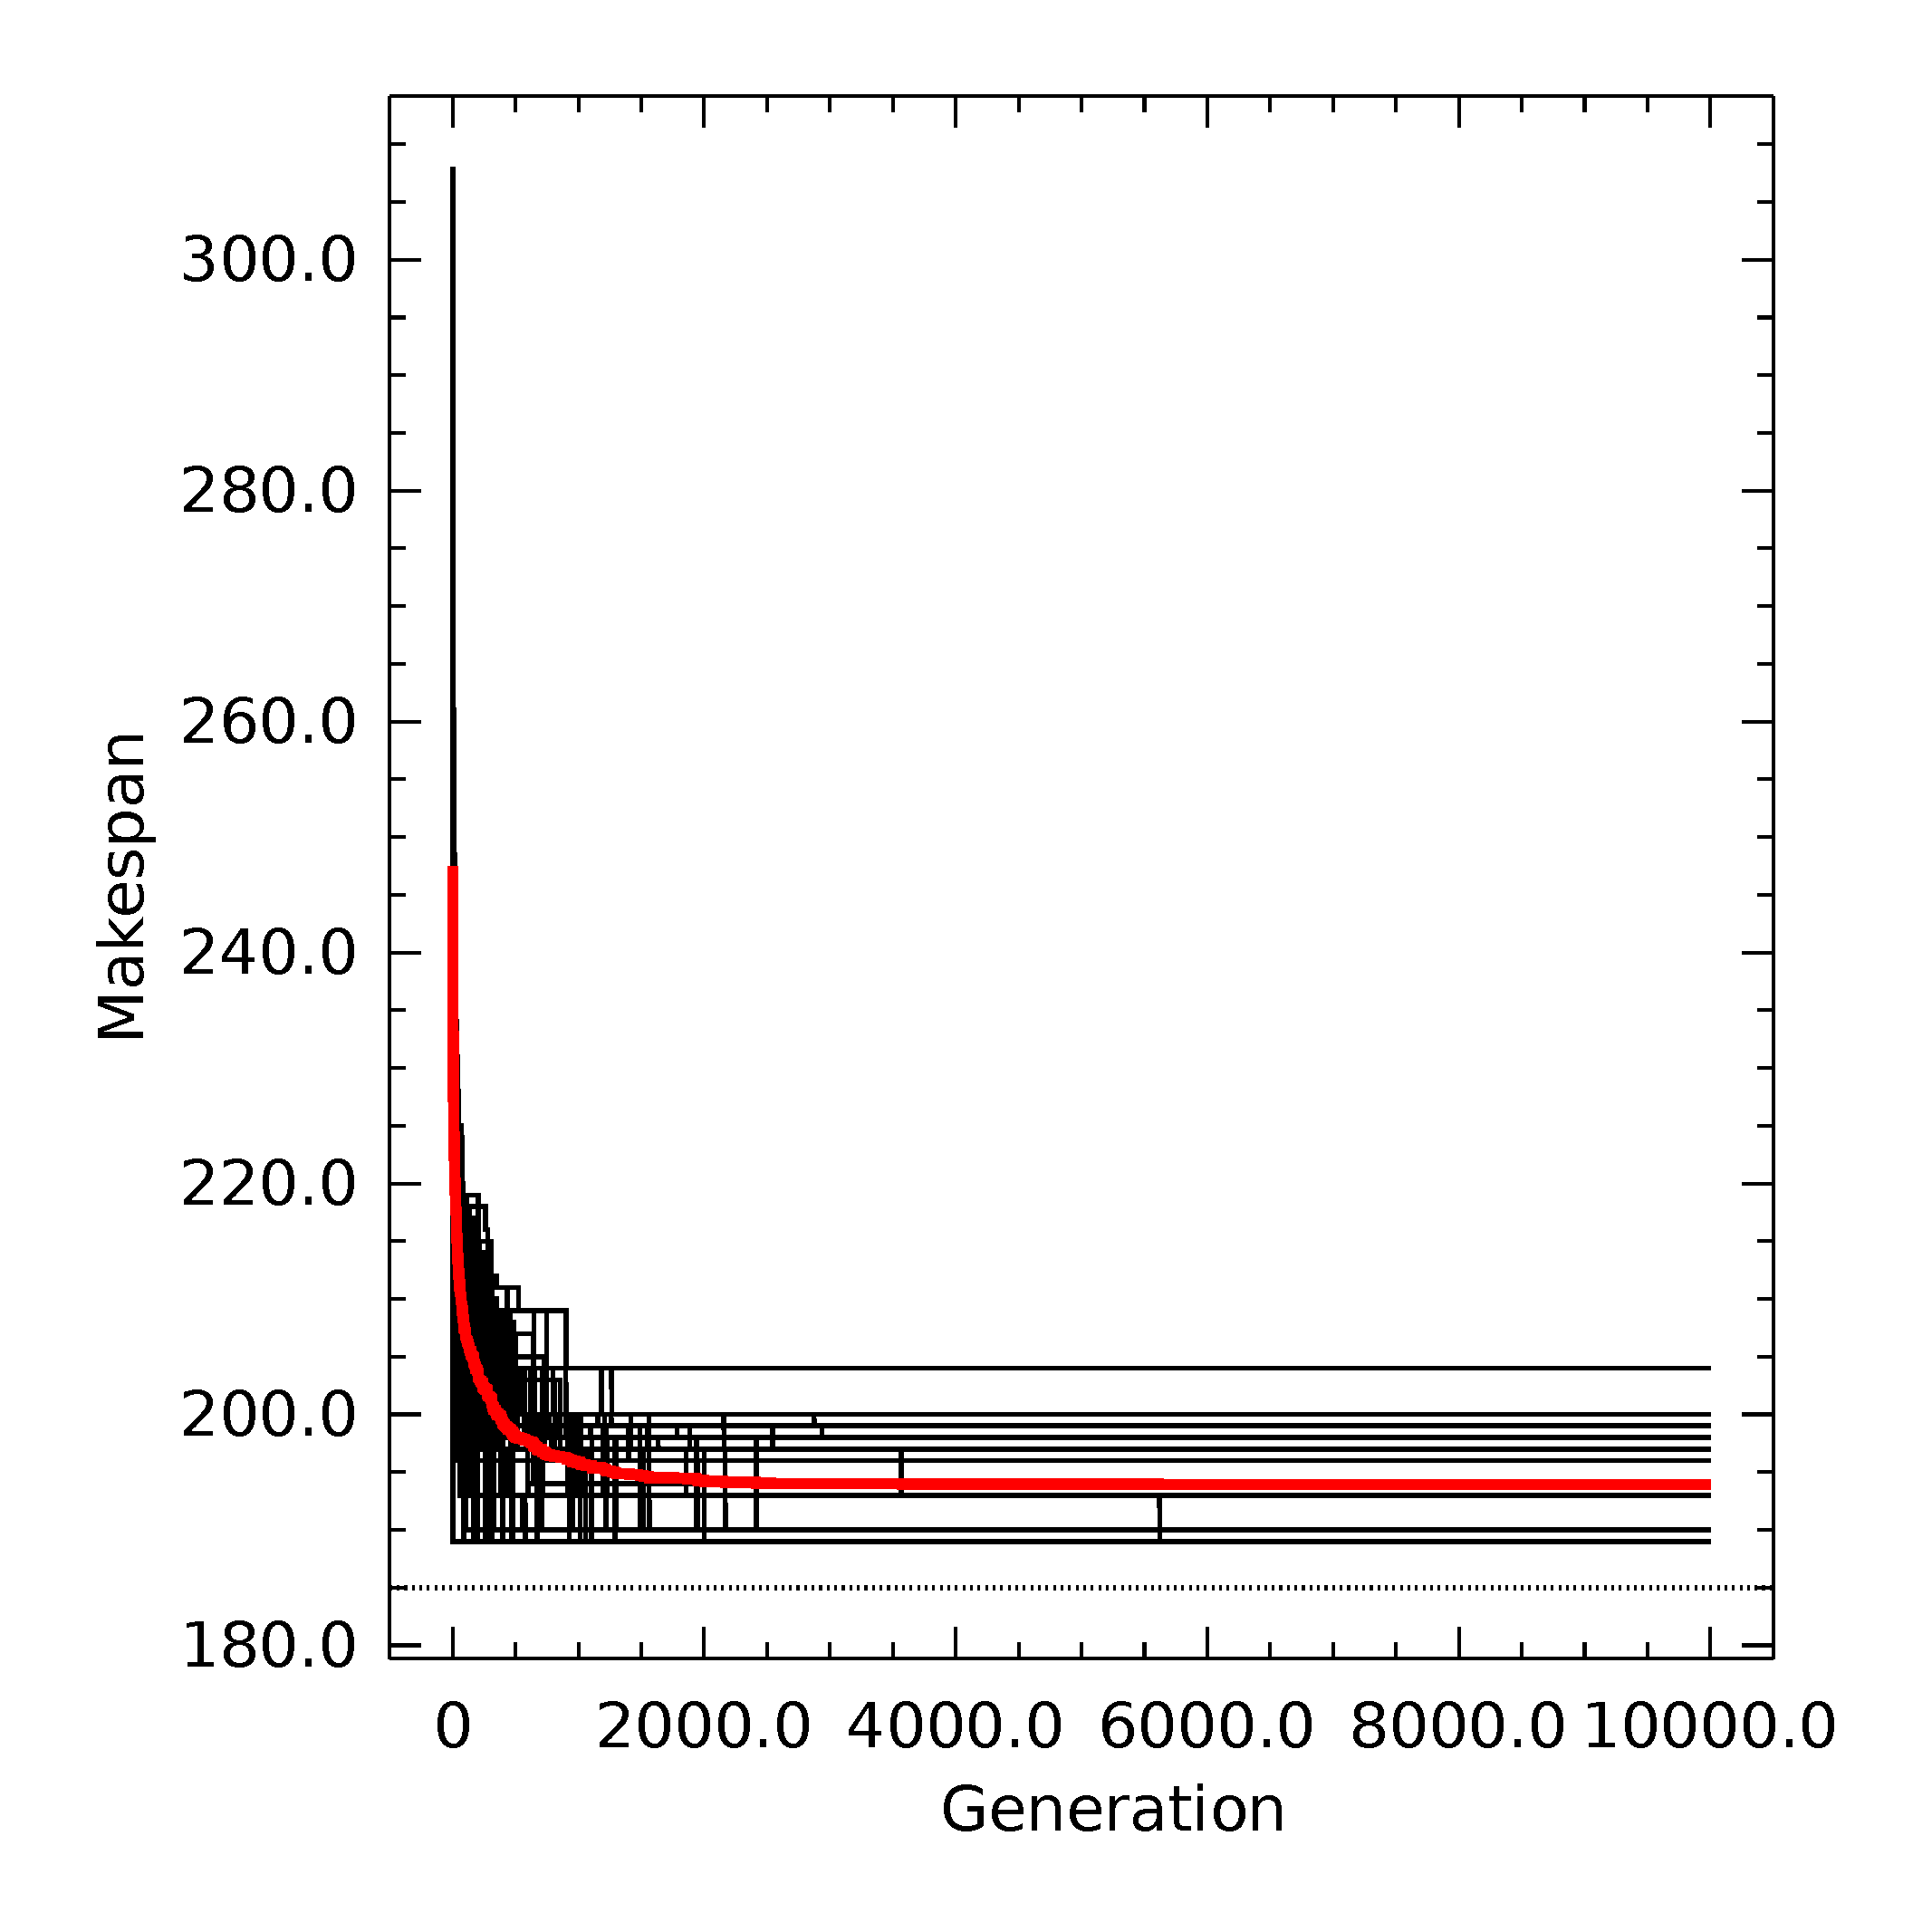
\includegraphics[scale=.095]{../open_jobshop/output/slf_4_6_10000.pdf}}
  \end{figure}
\end{frame}

\begin{frame}
  \frametitle{Convergence: 20x20 Problem}
  \begin{figure}[htbp]
    \centering
    \subfigure[Permutation GA]{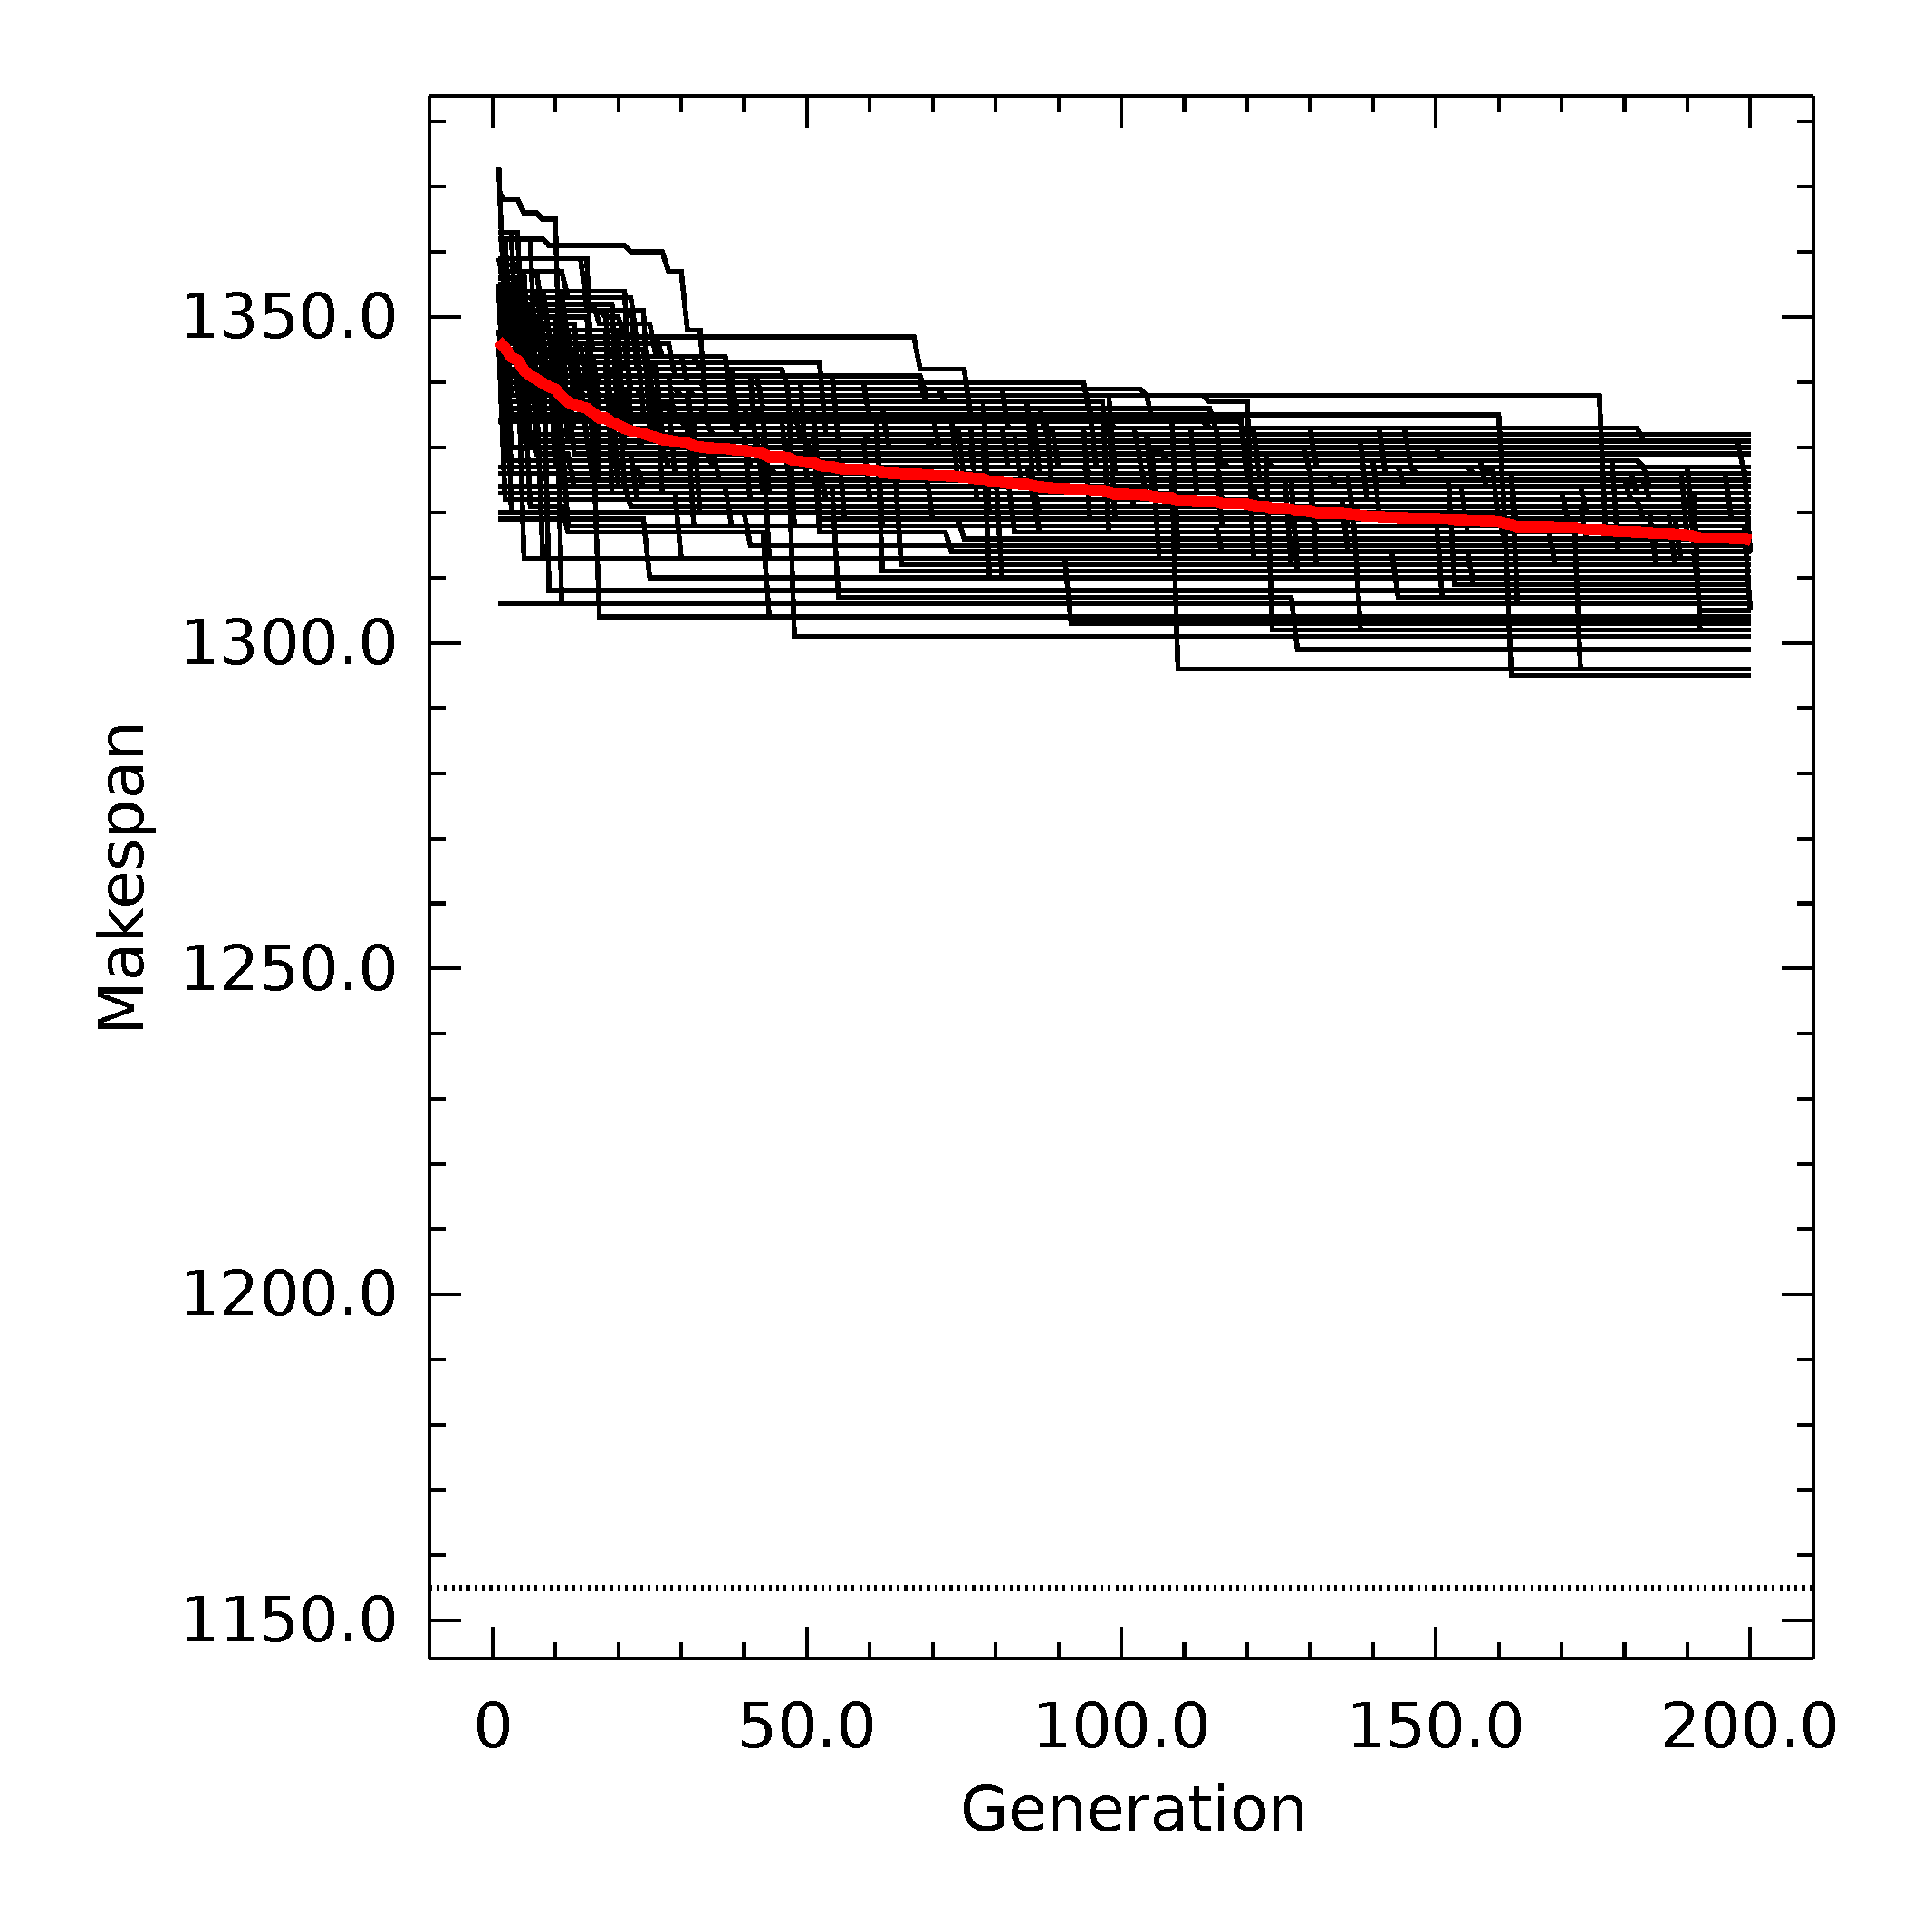
\includegraphics[scale=.095]{../open_jobshop/output/perm_20_1_200.pdf}}
    \subfigure[Hybrid GA]{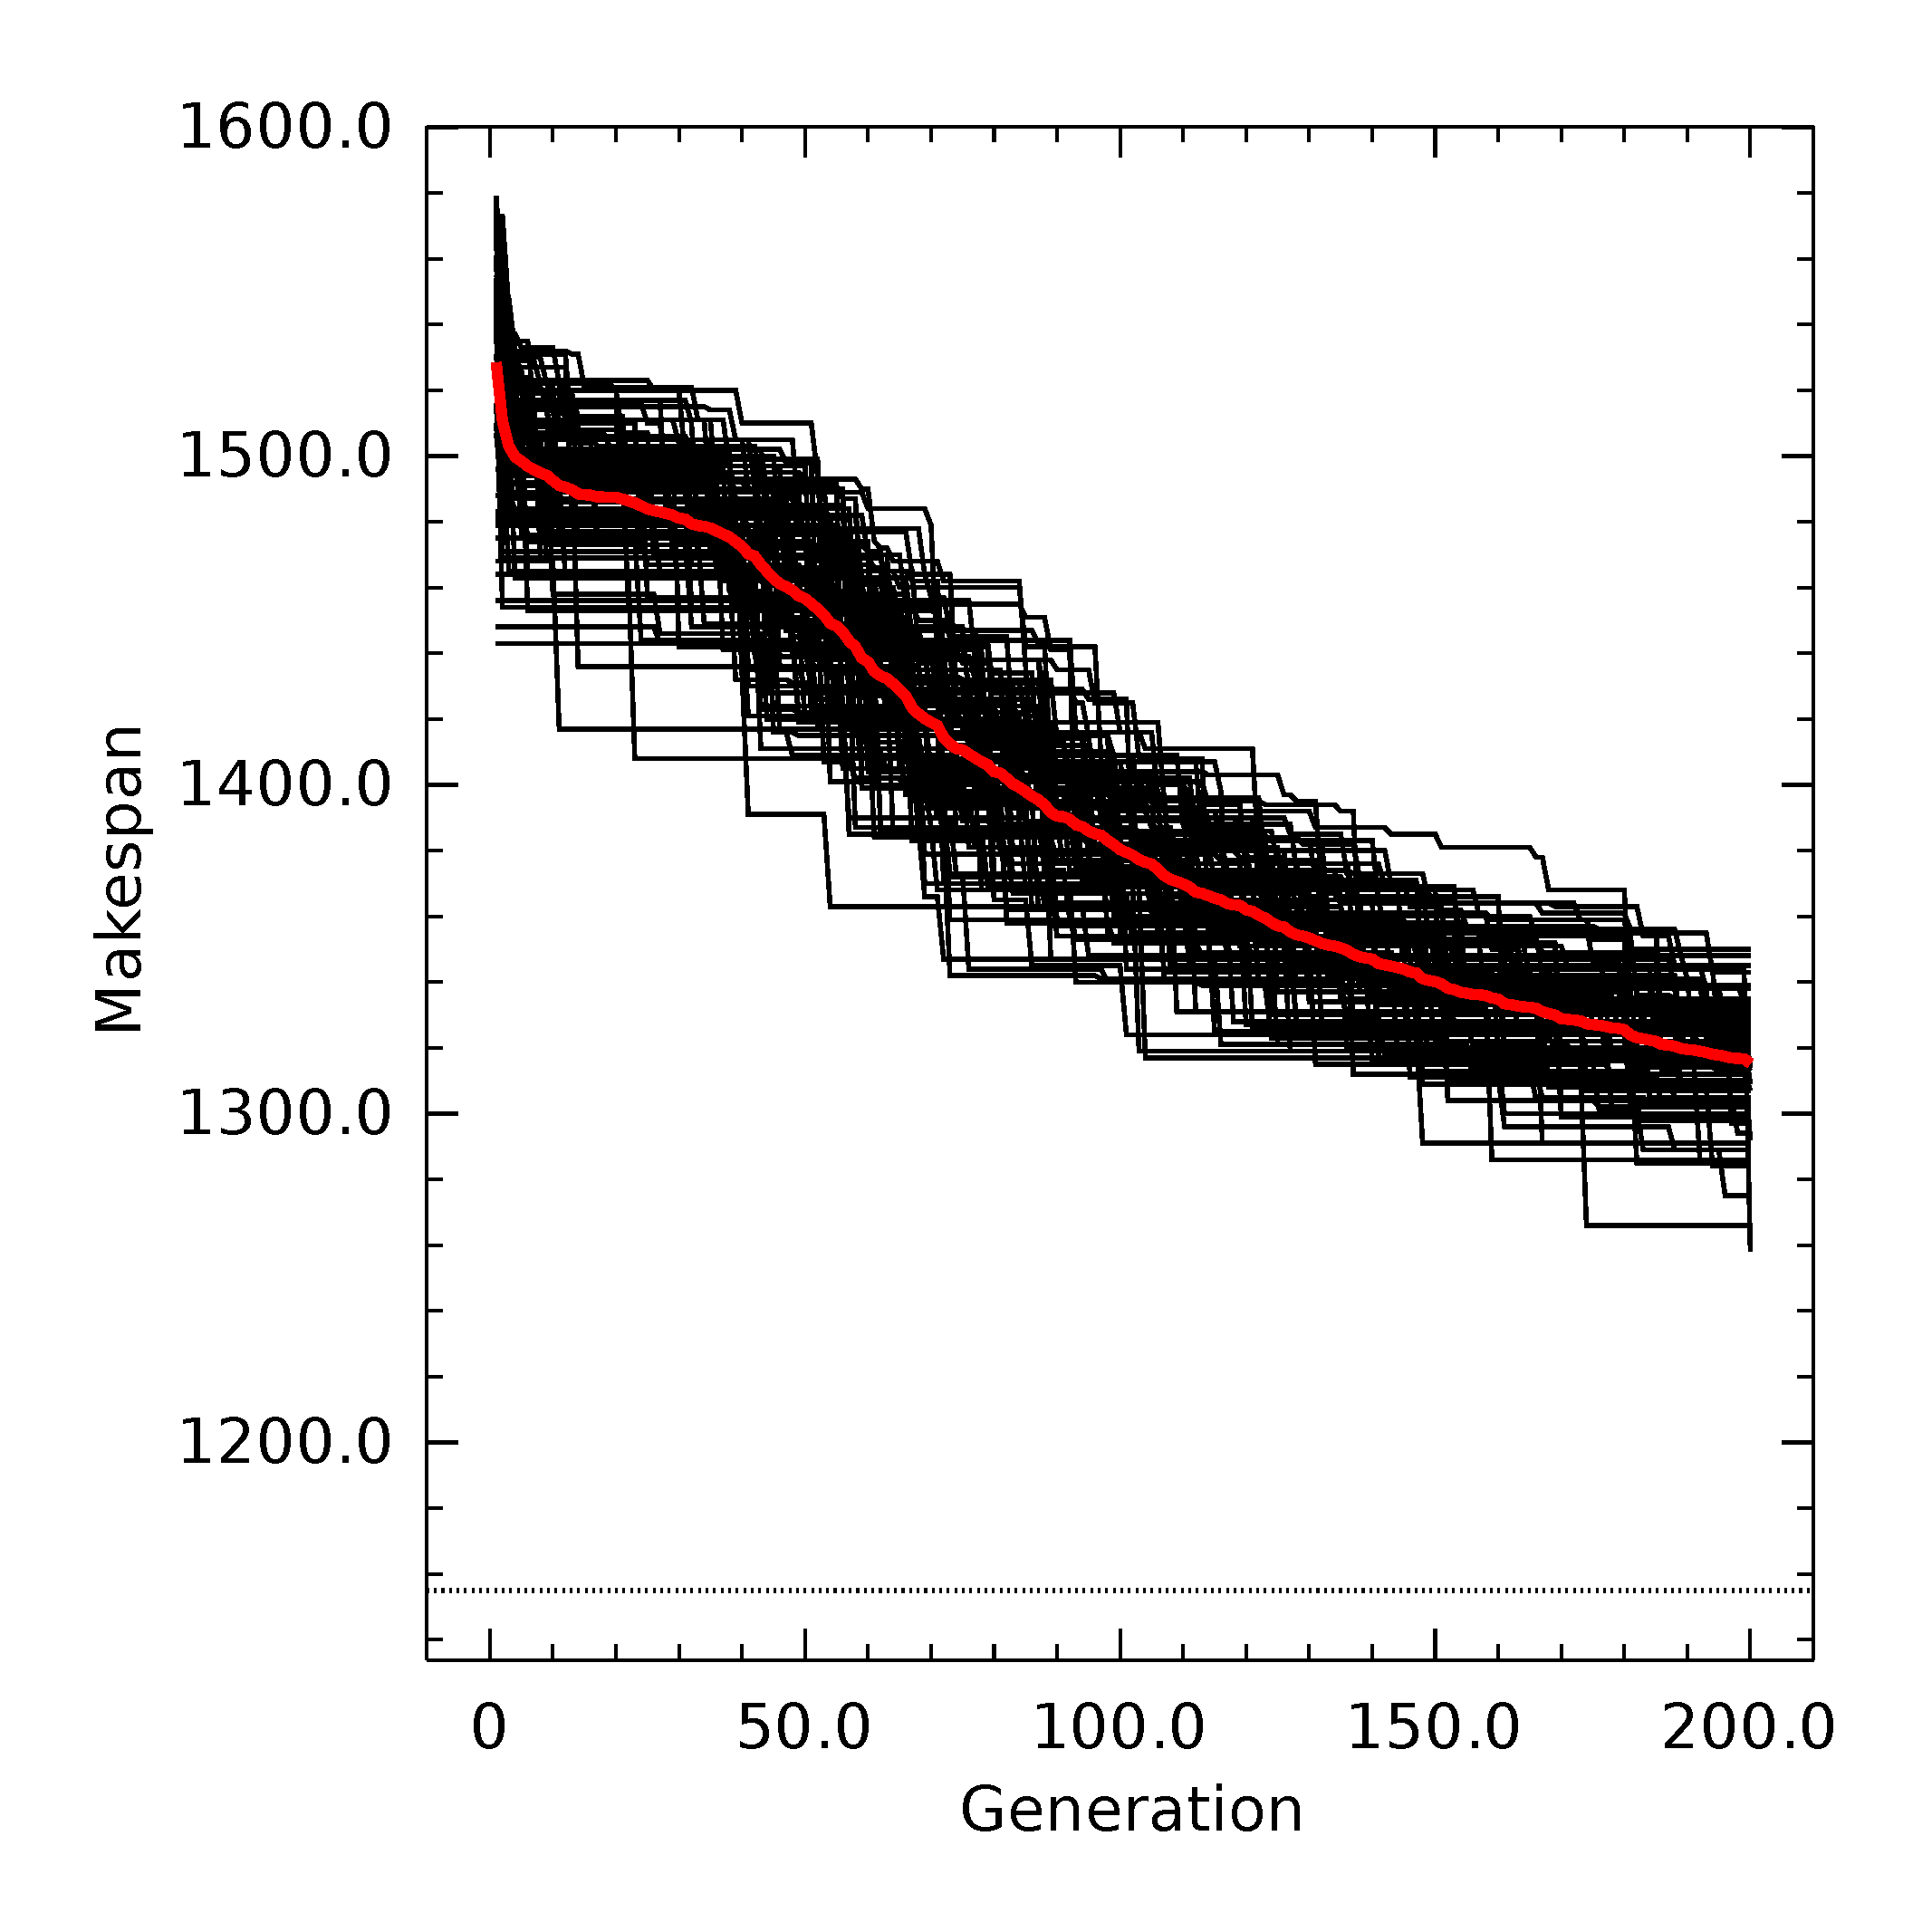
\includegraphics[scale=.095]{../open_jobshop/output/hyb_20_1_200.pdf}}
    \subfigure[Selfish Gene]{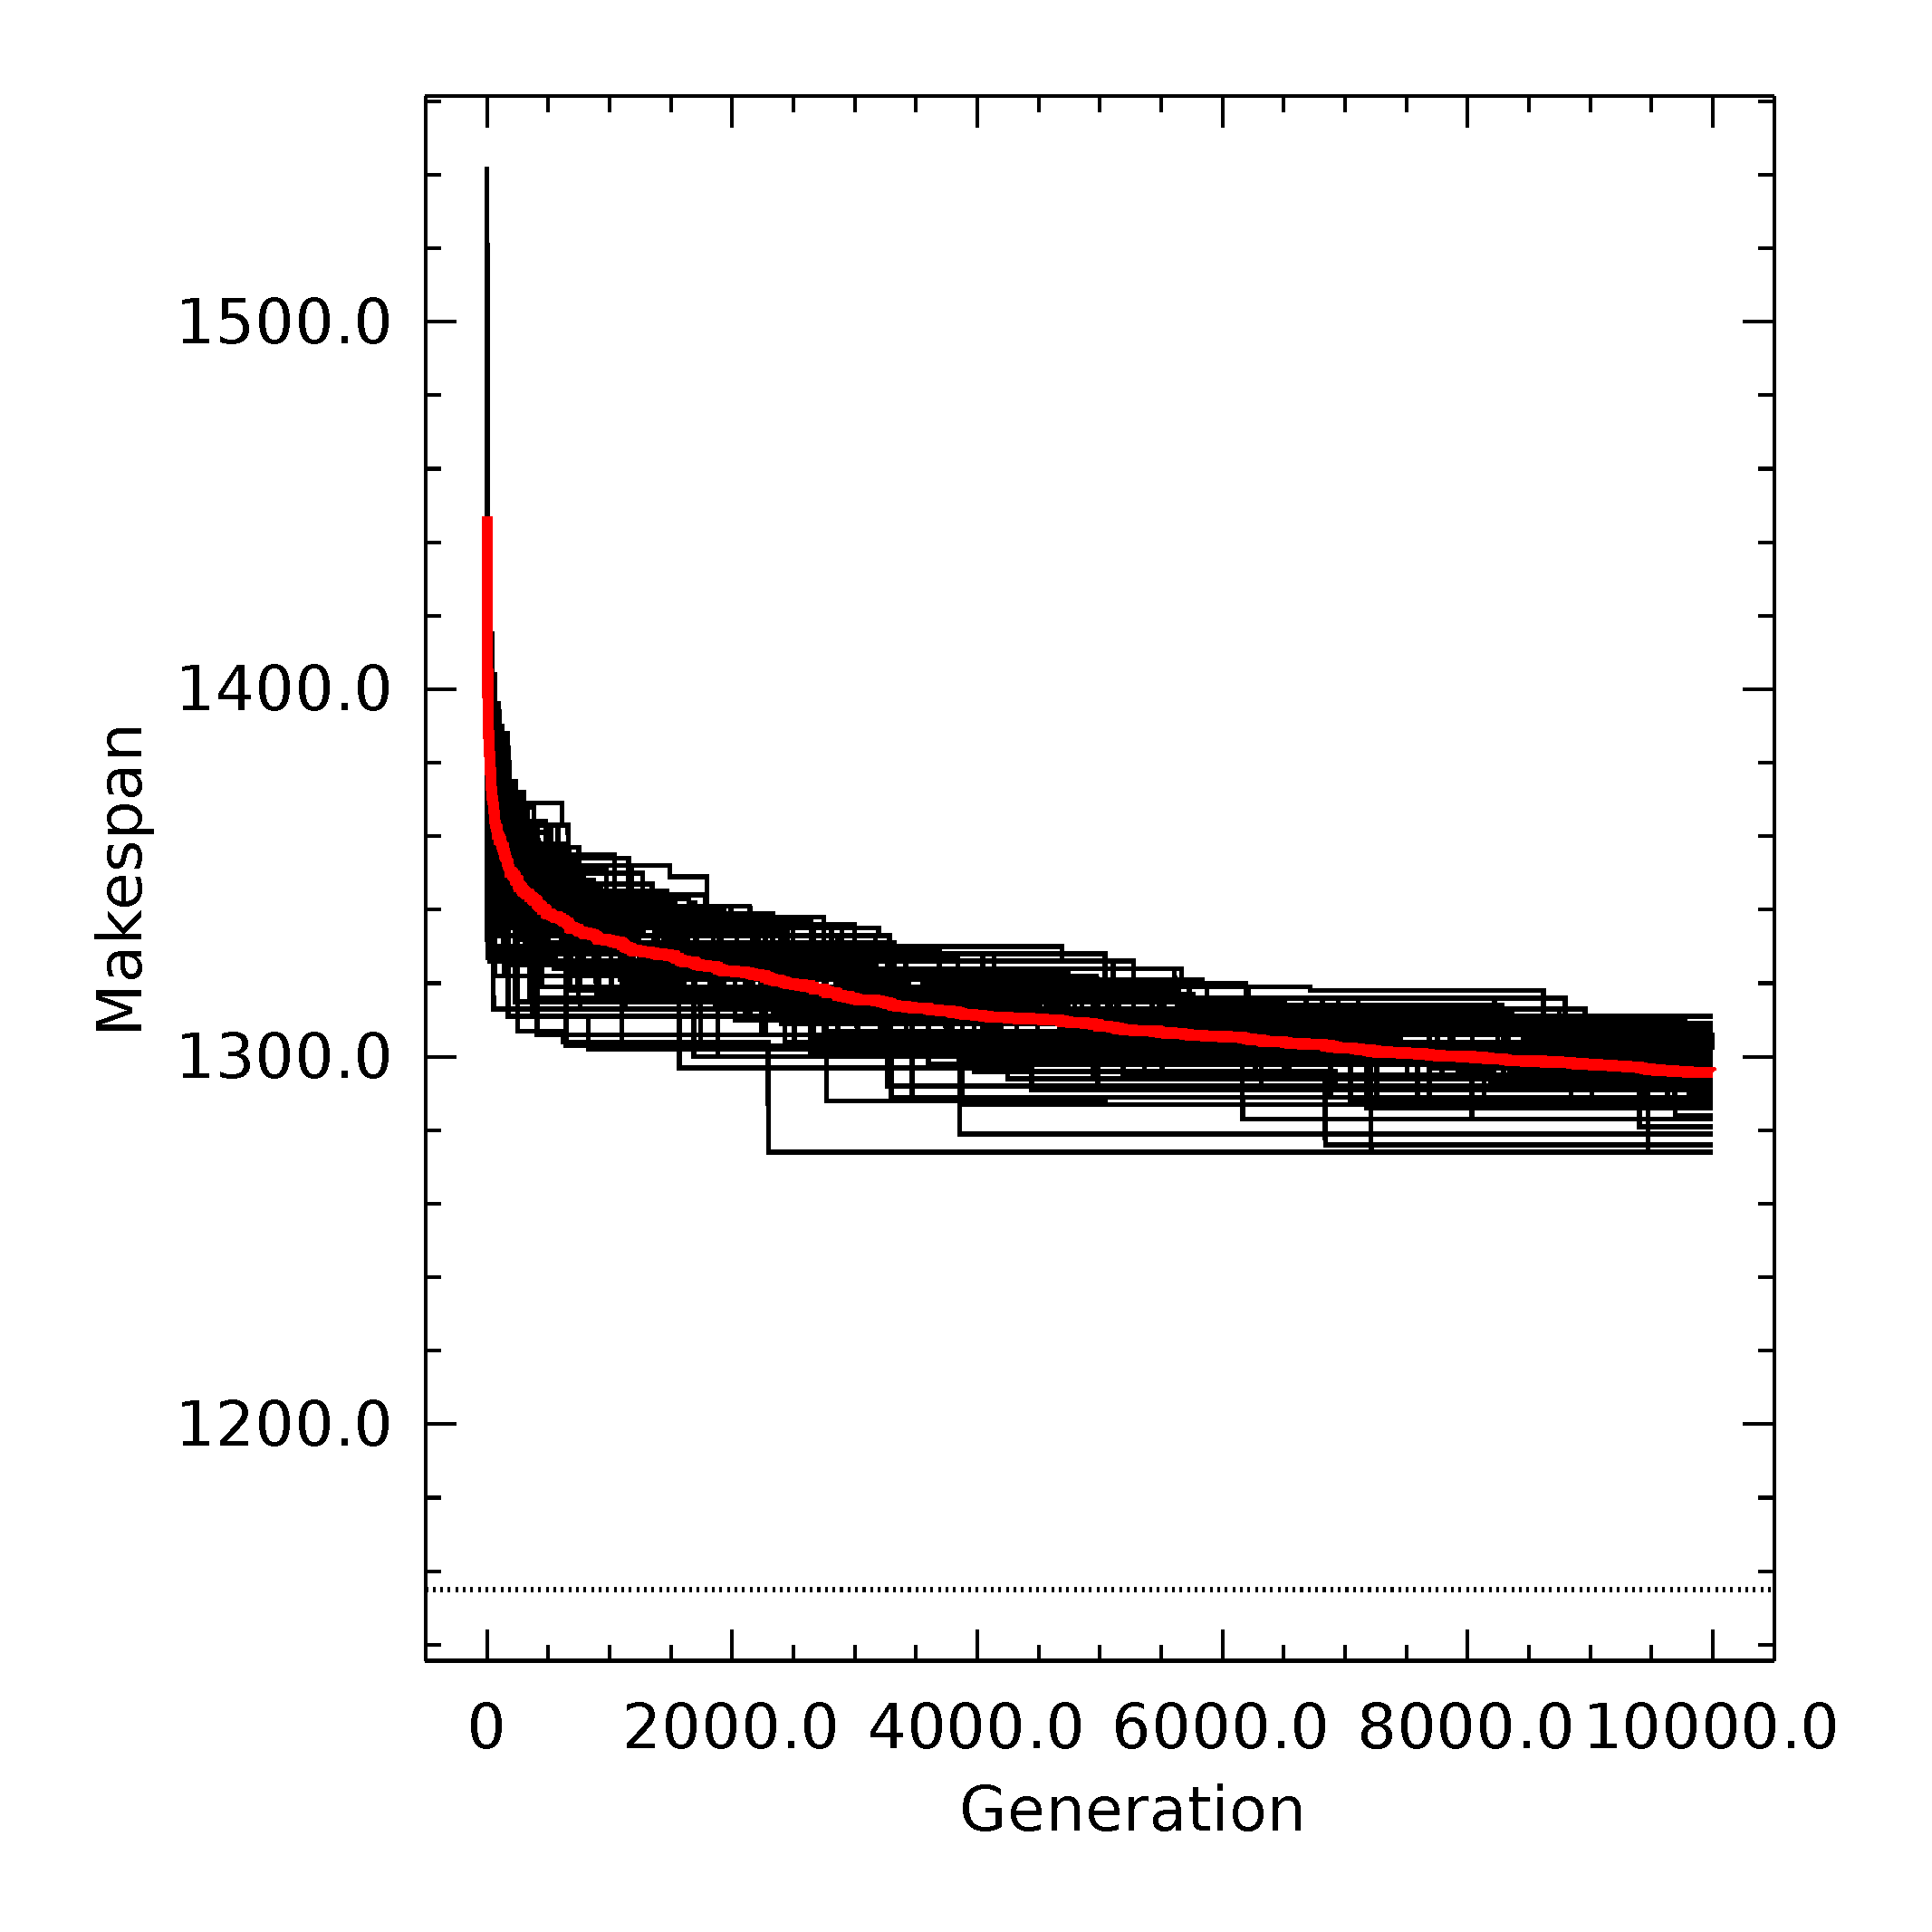
\includegraphics[scale=.095]{../open_jobshop/output/slf_20_1_10000.pdf}}
  \end{figure}
\end{frame}

%%%%%%%%%%%%%%%%%%%%%%%%%%%%%%%%%%%%%%%%%%%%%%%%%%%%%%%%%%%%%%%%%%%%%%%%%%%%%%%%




\section{Conclusion}
\subsection{nix}
\begin{frame}
  \frametitle{Conclusion}

  We

 \begin{itemize}
 
 	\item[\checkmark]  Implemented a general evolutionary library, capable of solving a wide range of problems,

 	\item[\checkmark]   thereby improving our understanding of the algorithms, 

 	\item[\checkmark]   applied it successfully to a well-known optimization problem,

 	\item[\checkmark]   got results comparable to earlier scientific research.
 \end{itemize}
 

%Possible Room for improvement: different crossover/mutation functions, computational efficiency, longer test runs




\end{frame}

\begin{frame}

\frametitle{References}
% 
 \small
 \bibliography{shortrefs}{}
 \bibliographystyle{ieeetr}
\end{frame}

%%%%%%%%%%%%%%%%%%%%%%%%%%%%%%%%%%%%%%%%%%%%%%%%%%%%%%%%%%%%%%%%%%%%%%%%%%%%
%\section{Beispiele}
%%%%%%%%%%%%%%%%%%%%%%%%%%%%%%%%%%%%%%%%%%%%%%%%%%%%%%%%%%%%%%%%%%%%%%%%%%%%%

%\subsection{Aufzählungen}
%\begin{frame}
	%\frametitle{Aufzählungen erstellen}
	%\begin{spacing}{1.5}
	%\begin{itemize}
		%\item Punkt 1
		%\begin{itemize}
			%\item Unterpunkt 1
			%\item Unterpunkt 2
		%\end{itemize}
		%\item Punkt 2
		%\item Punkt 3
	%\end{itemize}
	%\end{spacing}
%\end{frame}

%%%%%%%%%%%%%%%%%%%%%%%%%%%%%%%%%%%%%%%%%%%%%%%%%%%%%%%%%%%%%%%%%%%%%%%%%%%%%

%\subsection{Blöcke}
%\begin{frame}
	%\frametitle{Blöcke}
	%\framesubtitle{Normale Blöcke}
	%\begin{block}{Normaler Block}
		%Das ist ein Block mit einer Formel
		%\begin{eqnarray*}
		%u(x,t) & = & \sum_{k=1}^{\infty} f_k \sin \frac{k \pi x}{L} \cos 
					 %\frac{k \pi t}{aL} + \\
				 %& + & \sum_{k=1}^{\infty} g_k \sin \frac{k \pi x}{L} \sin 
					 %\frac{k \pi t}{aL} \\
		%\end{eqnarray*}
	%\end{block}
%\end{frame}

%%%%%%%%%%%%%%%%%%%%%%%%%%%%%%%%%%%%%%%%%%%%%%%%%%%%%%%%%%%%%%%%%%%%%%%%%%%%%

%\begin{frame}[fragile]
	%\frametitle{Blöcke}
	%\framesubtitle{Beispiel-Blöcke}
	%\begin{exampleblock}{Beispiel-Block}
	%\begin{semiverbatim}
%SUCHE (A,x)
%1: i = 0
%2: WHILE i<n
%3:     i = i+1
%4:     \alert{IF A[i]=x THEN RETURN i}
%5: ELSE RETURN -1
	%\end{semiverbatim}
	%\end{exampleblock}
%\end{frame}

%%%%%%%%%%%%%%%%%%%%%%%%%%%%%%%%%%%%%%%%%%%%%%%%%%%%%%%%%%%%%%%%%%%%%%%%%%%%%

%\begin{frame}
	%\frametitle{Blöcke}
	%\framesubtitle{Alert-Blöcke}
	%\Large
	%\begin{alertblock}{Alert-Block}
		%\centering
		%Achtung! Nicht zu viel Inhalt auf eine Folie!
	%\end{alertblock}
%\end{frame}

%%%%%%%%%%%%%%%%%%%%%%%%%%%%%%%%%%%%%%%%%%%%%%%%%%%%%%%%%%%%%%%%%%%%%%%%%%%%%

%\subsection{Spalten und Grafiken}
%\begin{frame}
	%\frametitle{Spalten und Grafiken}
	%\begin{columns}
		%\begin{column}{0.5\textwidth}
			%Aufzählung in Spalte 1
			%\begin{enumerate}
				%\item Punkt 1
				%\item Punkt 2
				%\item Punkt 3
			%\end{enumerate}
		%\end{column}
		%\begin{column}{0.5\textwidth}
			%\begin{center}
			%%\includegraphics[width=0.4\textwidth]{smail}

			%Grafik in Spalte 2
			%\end{center}
		%\end{column}
	%\end{columns}
%\end{frame}

%%%%%%%%%%%%%%%%%%%%%%%%%%%%%%%%%%%%%%%%%%%%%%%%%%%%%%%%%%%%%%%%%%%%%%%%%%%%%
%\section{Abschnitt 2}
%%%%%%%%%%%%%%%%%%%%%%%%%%%%%%%%%%%%%%%%%%%%%%%%%%%%%%%%%%%%%%%%%%%%%%%%%%%%%

%%%%%%%%%%%%%%%%%%%%%%%%%%%%%%%%%%%%%%%%%%%%%%%%%%%%%%%%%%%%%%%%%%%%%%%%%%%%%
%\section{Abschnitt 3}
%%%%%%%%%%%%%%%%%%%%%%%%%%%%%%%%%%%%%%%%%%%%%%%%%%%%%%%%%%%%%%%%%%%%%%%%%%%%%

%%%%%%%%%%%%%%%%%%%%%%%%%%%%%%%%%%%%%%%%%%%%%%%%%%%%%%%%%%%%%%%%%%%%%%%%%%%%%
%\section{Zusammenfassung}
%%%%%%%%%%%%%%%%%%%%%%%%%%%%%%%%%%%%%%%%%%%%%%%%%%%%%%%%%%%%%%%%%%%%%%%%%%%%%

%\begin{frame}
	%\frametitle{Zusammenfassung}
	%\begin{itemize}
		%\item Punkt 1
		%\item Punkt 2
		%\item Punkt 3
	%\end{itemize}
%\end{frame}


%%%%%%%%%%%%%%%%%%%%%%%%%%%%%%%%%%%%%%%%%%%%%%%%%%%%%%%%%%%%%%%%%%%%%%%%%%%%%
%\section*{} % Damit die Kontakt-Folie nicht im Inhaltsverzeichnis aufscheint
%%%%%%%%%%%%%%%%%%%%%%%%%%%%%%%%%%%%%%%%%%%%%%%%%%%%%%%%%%%%%%%%%%%%%%%%%%%%%

%\begin{frame}
%\frametitle{Kontakt}
%nothing
%\end{frame}

%%%%%%%%%%%%%%%%%%%%%%%%%%%%%%%%%%%%%%%%%%%%%%%%%%%%%%%%%%%%%%%%%%%%%%%%%%%%
\end{document}
%%%%%%%%%%%%%%%%%%%%%%%%%%%%%%%%%%%%%%%%%%%%%%%%%%%%%%%%%%%%%%%%%%%%%%%%%%%%

%% EOF
